\section{Apêndices}
\subsection{Apêndice A}
\begin{table}[H]
    \centering
    \caption{Levantamento das edificações de escritório de Vitória.}
    \begin{tabular}{l}
        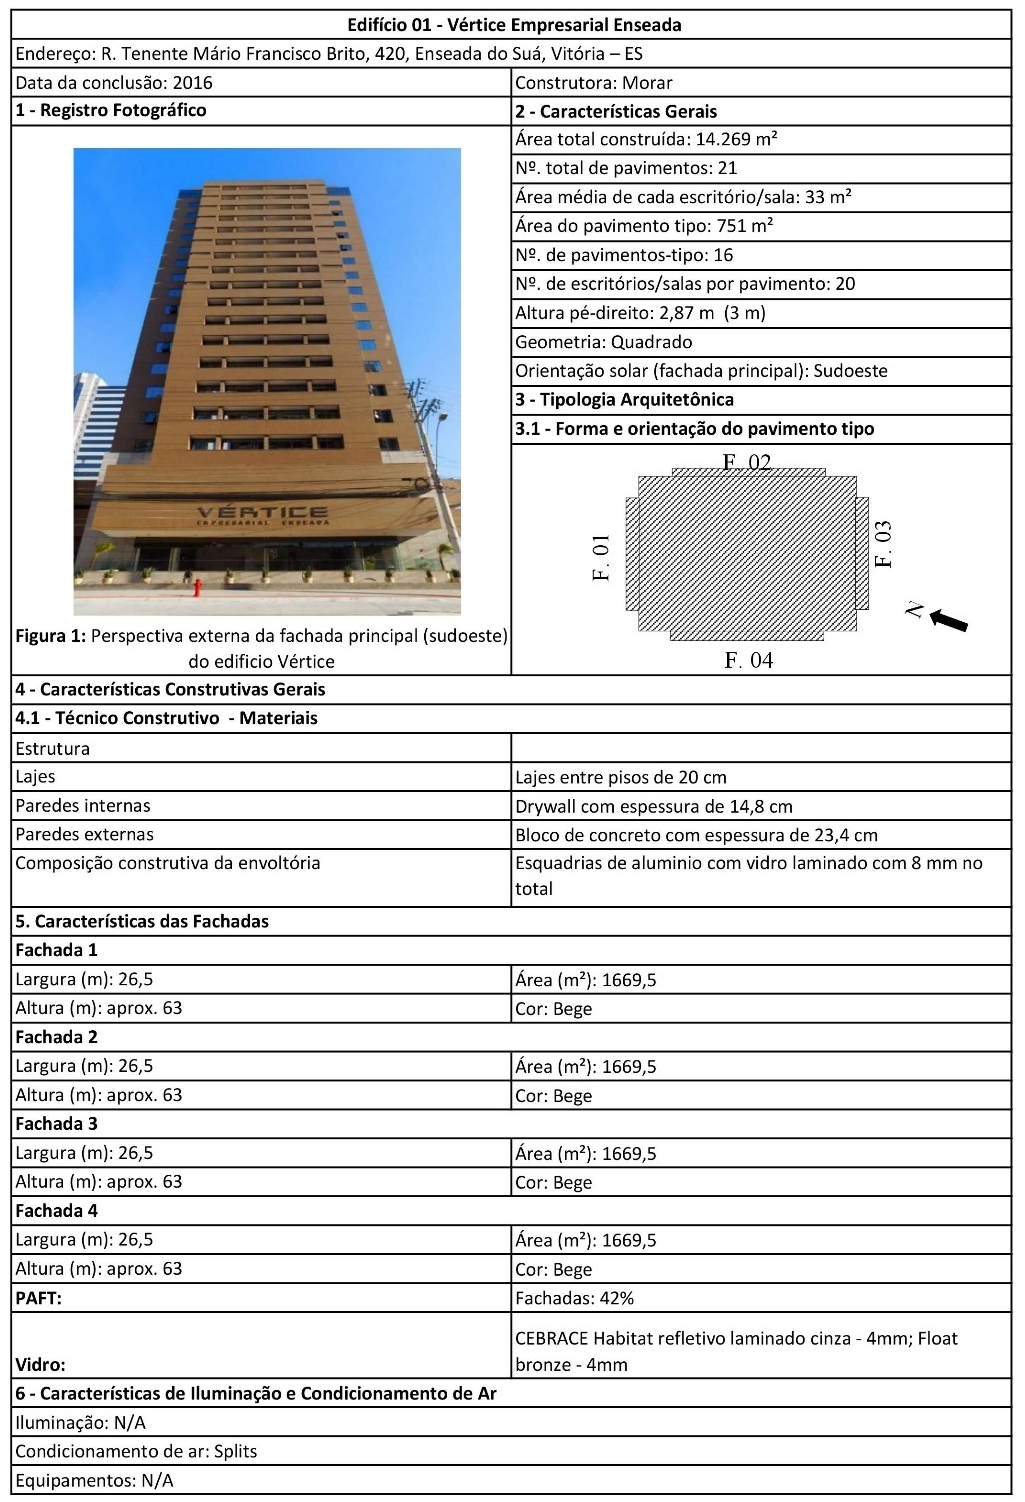
\includegraphics[width=0.9\textwidth]{figures/appendices/edificio01.png}
    \end{tabular}
    \label{tab:18}
\end{table}
\pagebreak
\begin{table}[H]
    \centering
    \begin{tabular}{l}
        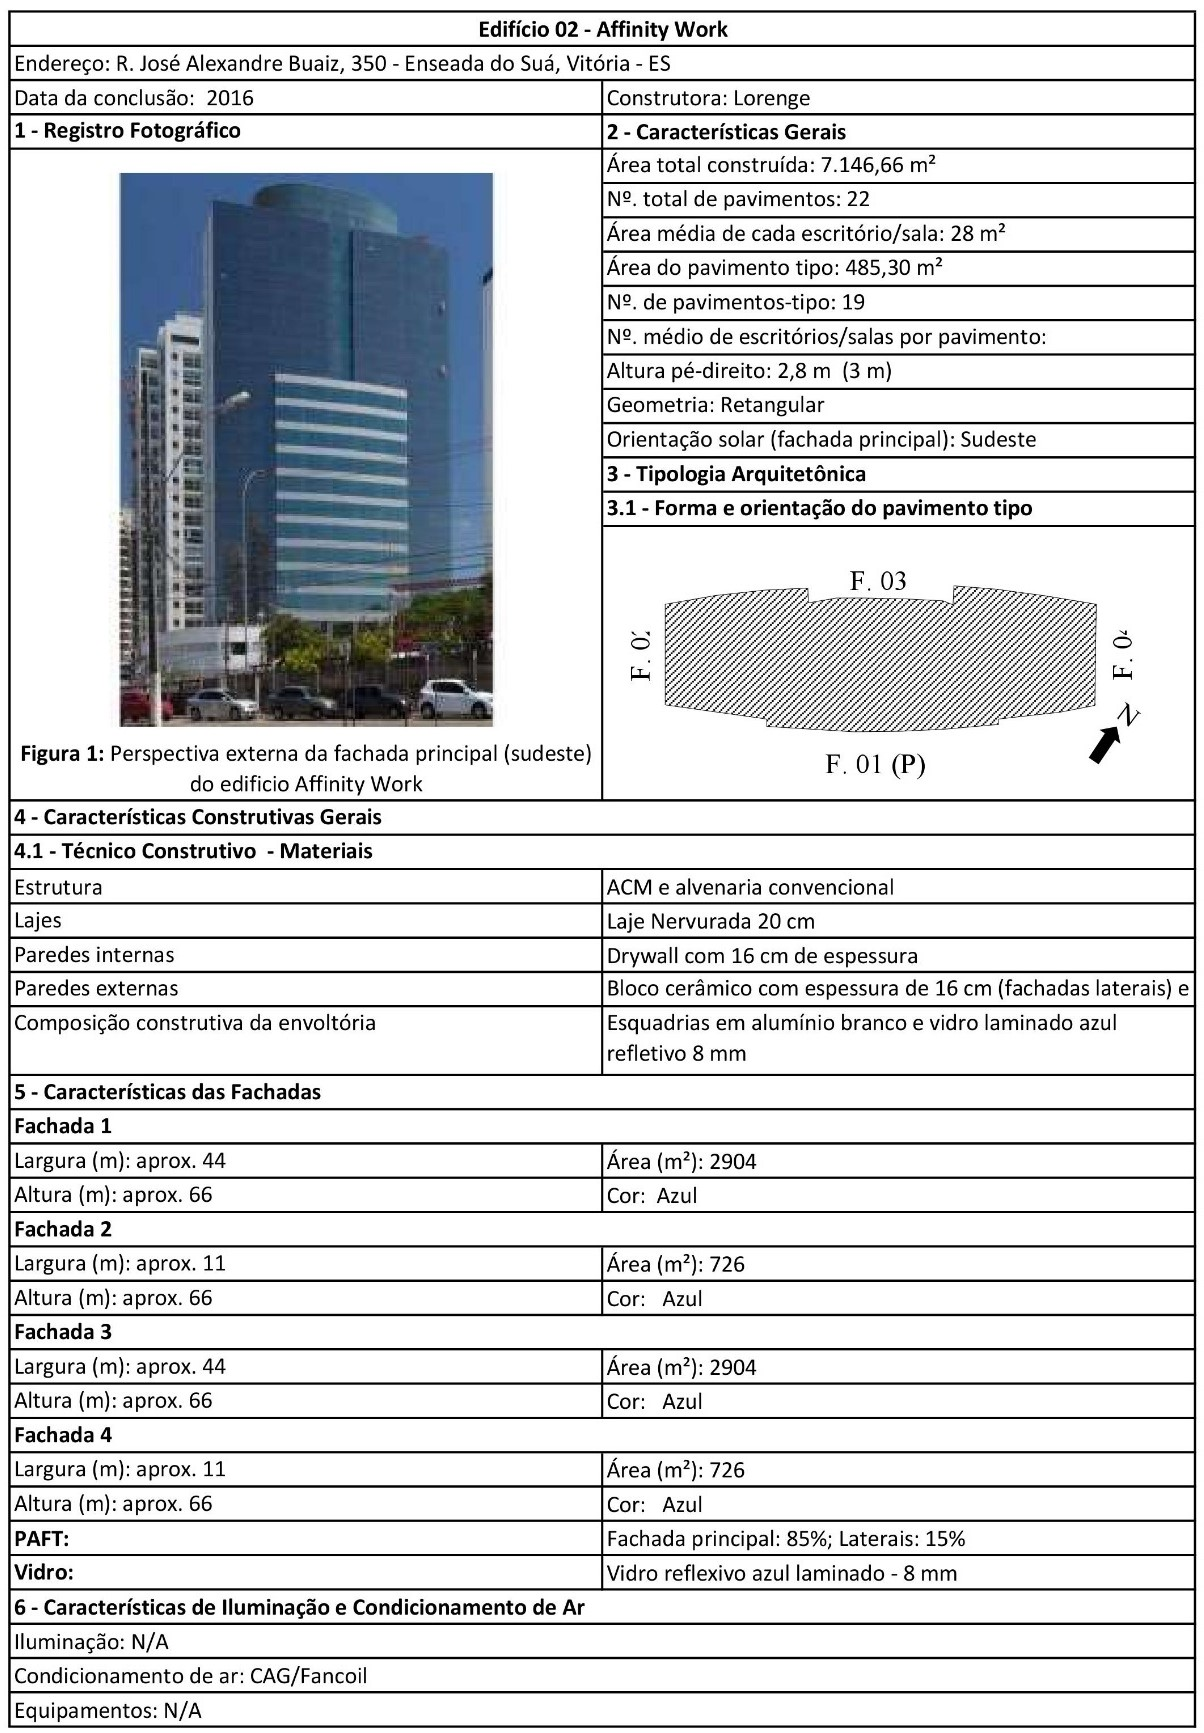
\includegraphics[width=\textwidth]{figures/appendices/edificio02.jpg}
    \end{tabular}
\end{table}
\pagebreak
\begin{table}[H]
    \centering
    \begin{tabular}{l}
        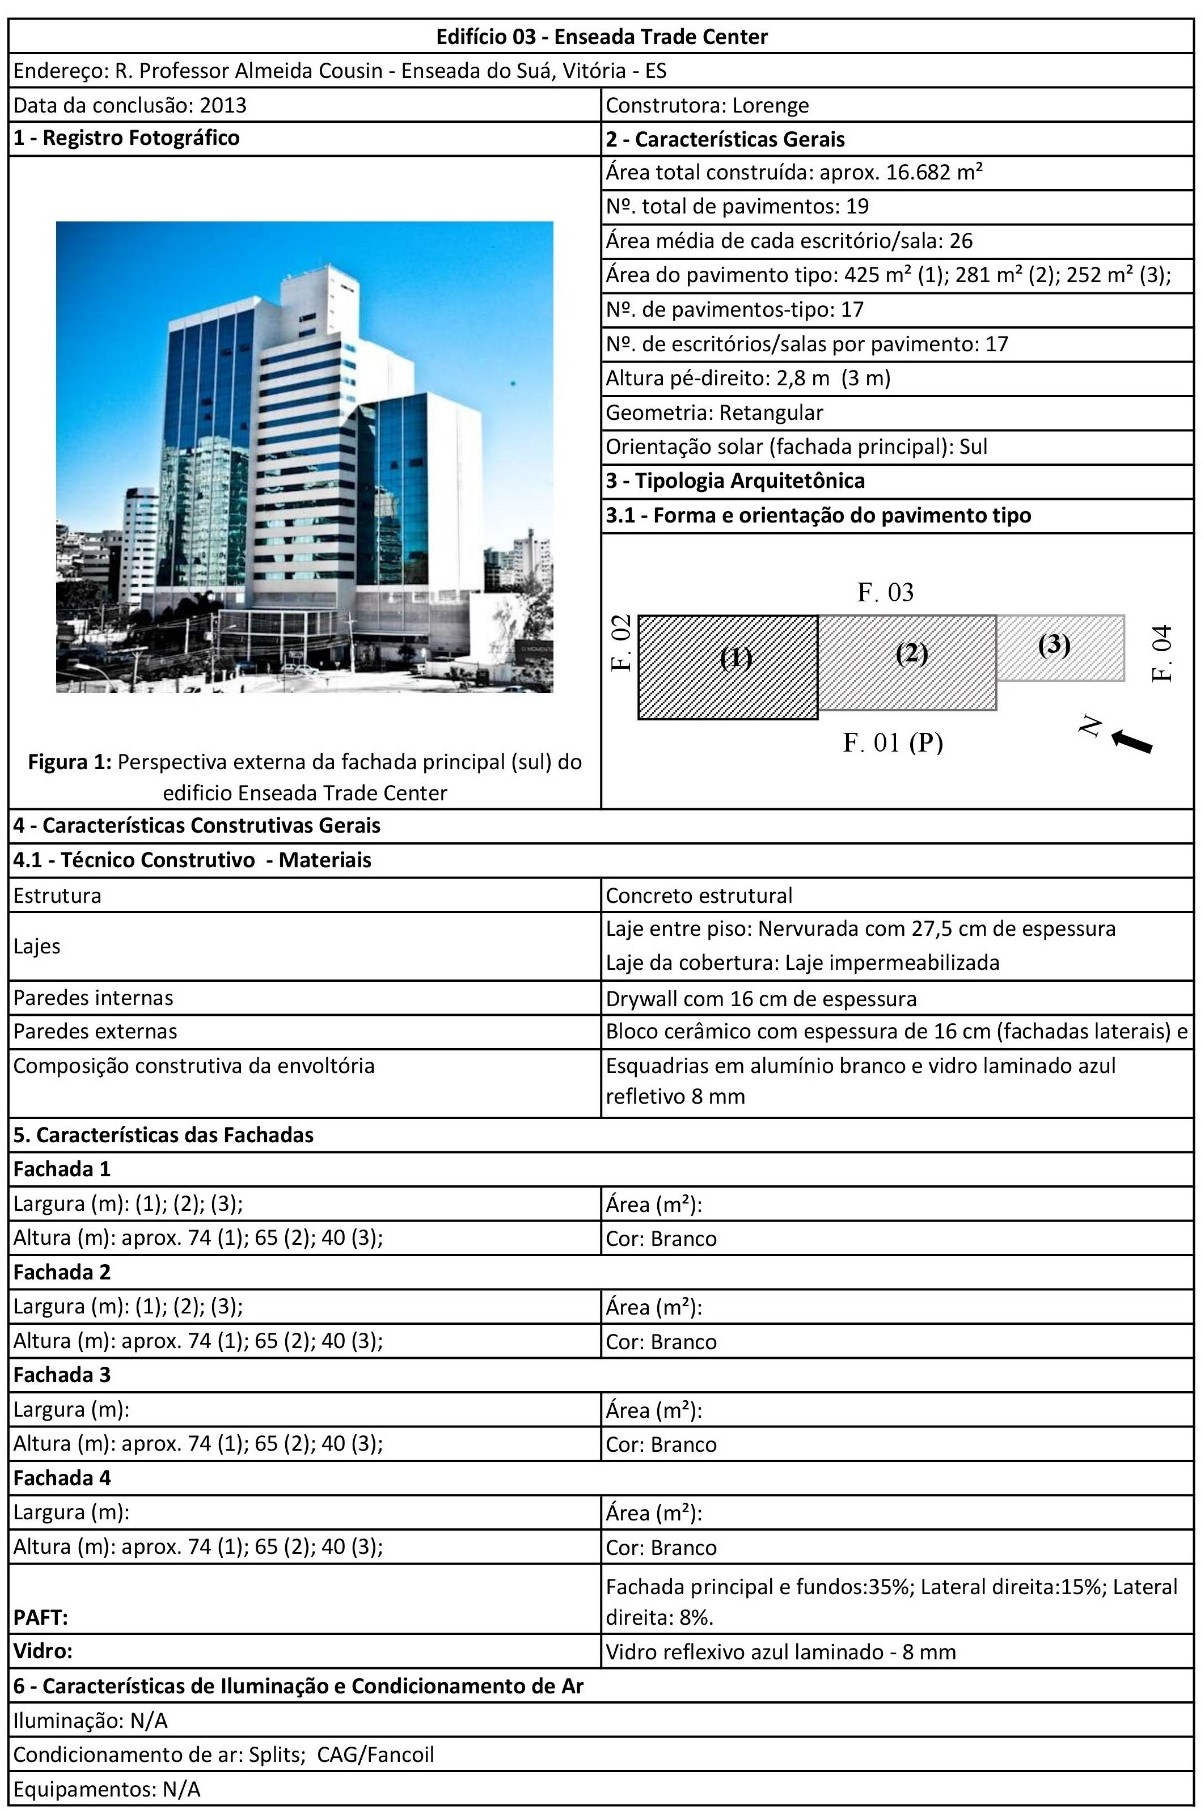
\includegraphics[width=\textwidth]{figures/appendices/edificio03.jpg}
    \end{tabular}
\end{table}
\pagebreak
\begin{table}[H]
    \centering
    \begin{tabular}{l}
        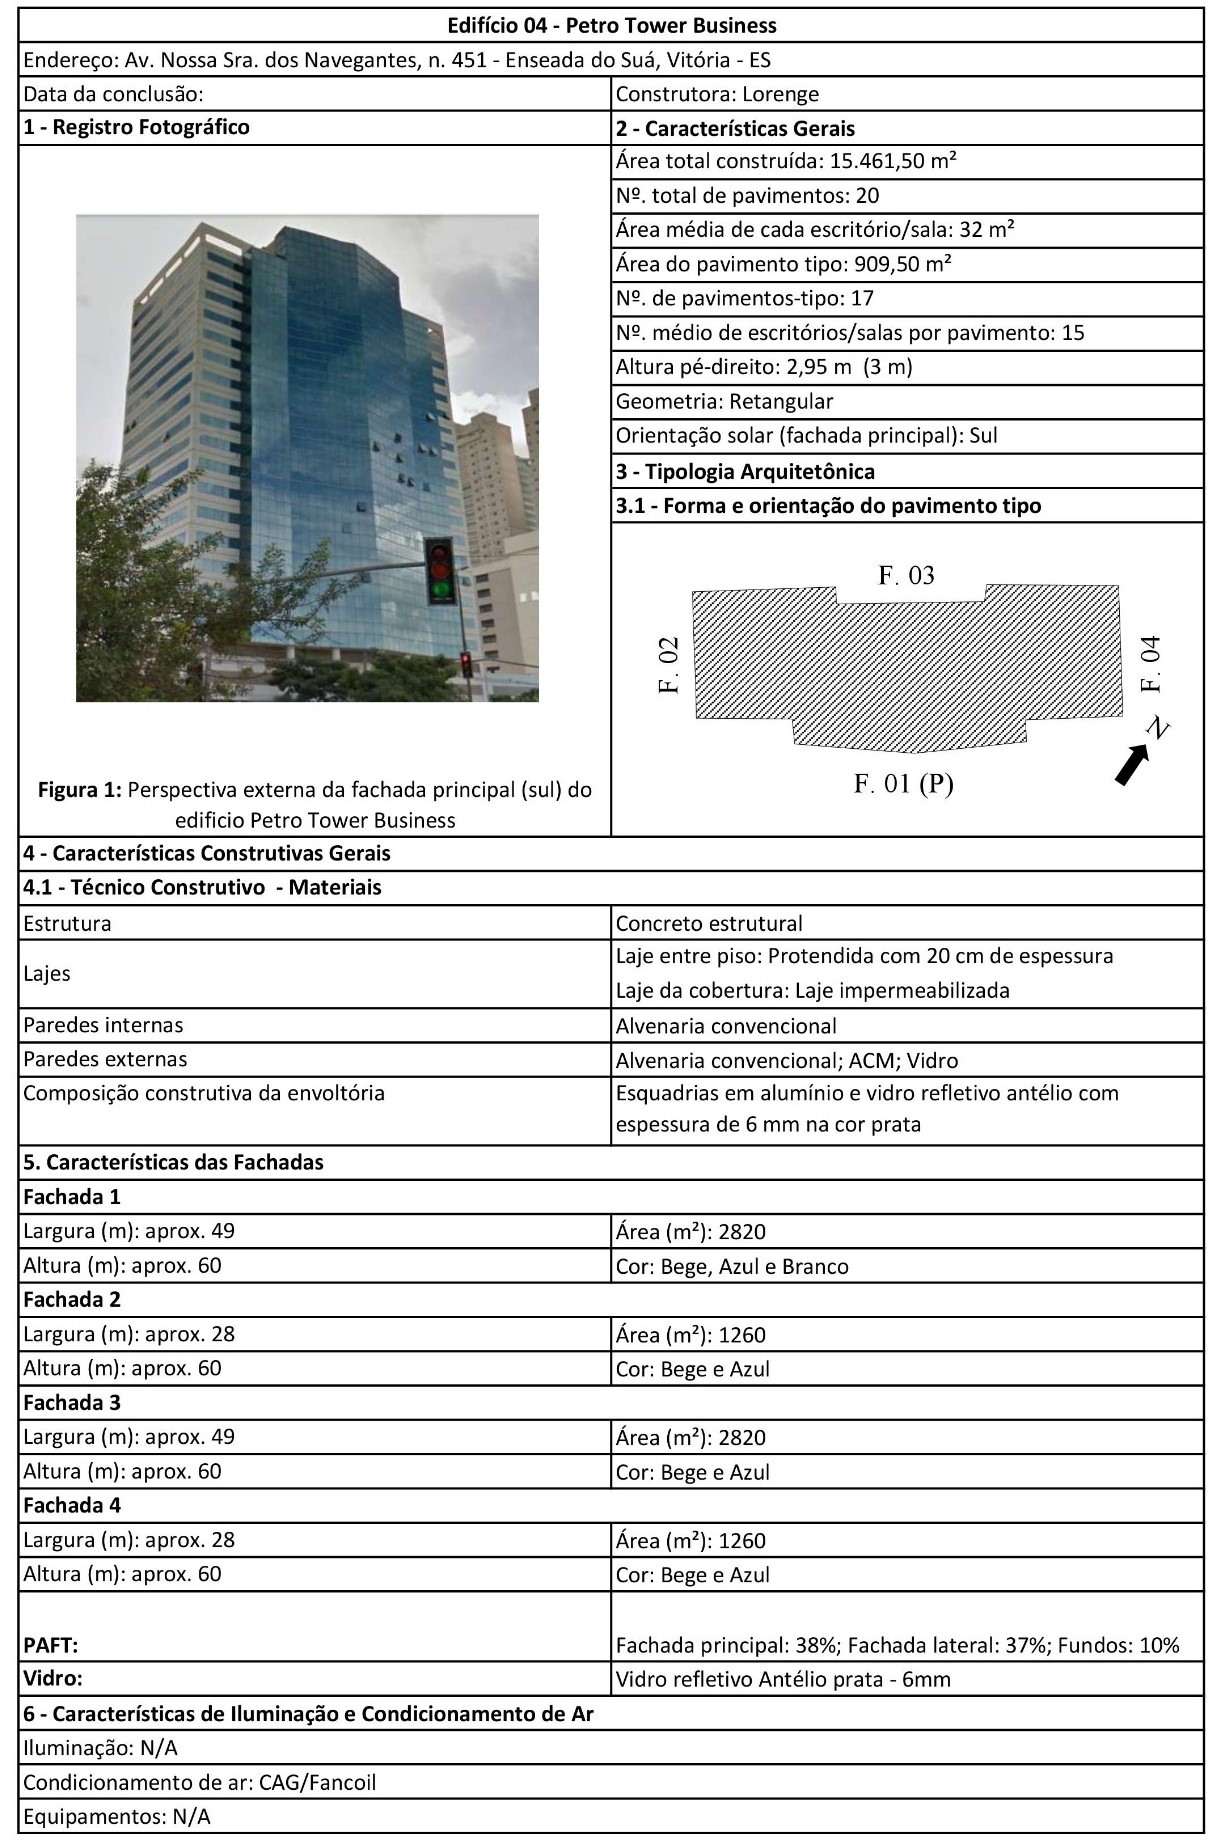
\includegraphics[width=\textwidth]{figures/appendices/edificio04.jpg}
    \end{tabular}
\end{table}
\pagebreak
\begin{table}[H]
    \centering
    \begin{tabular}{l}
        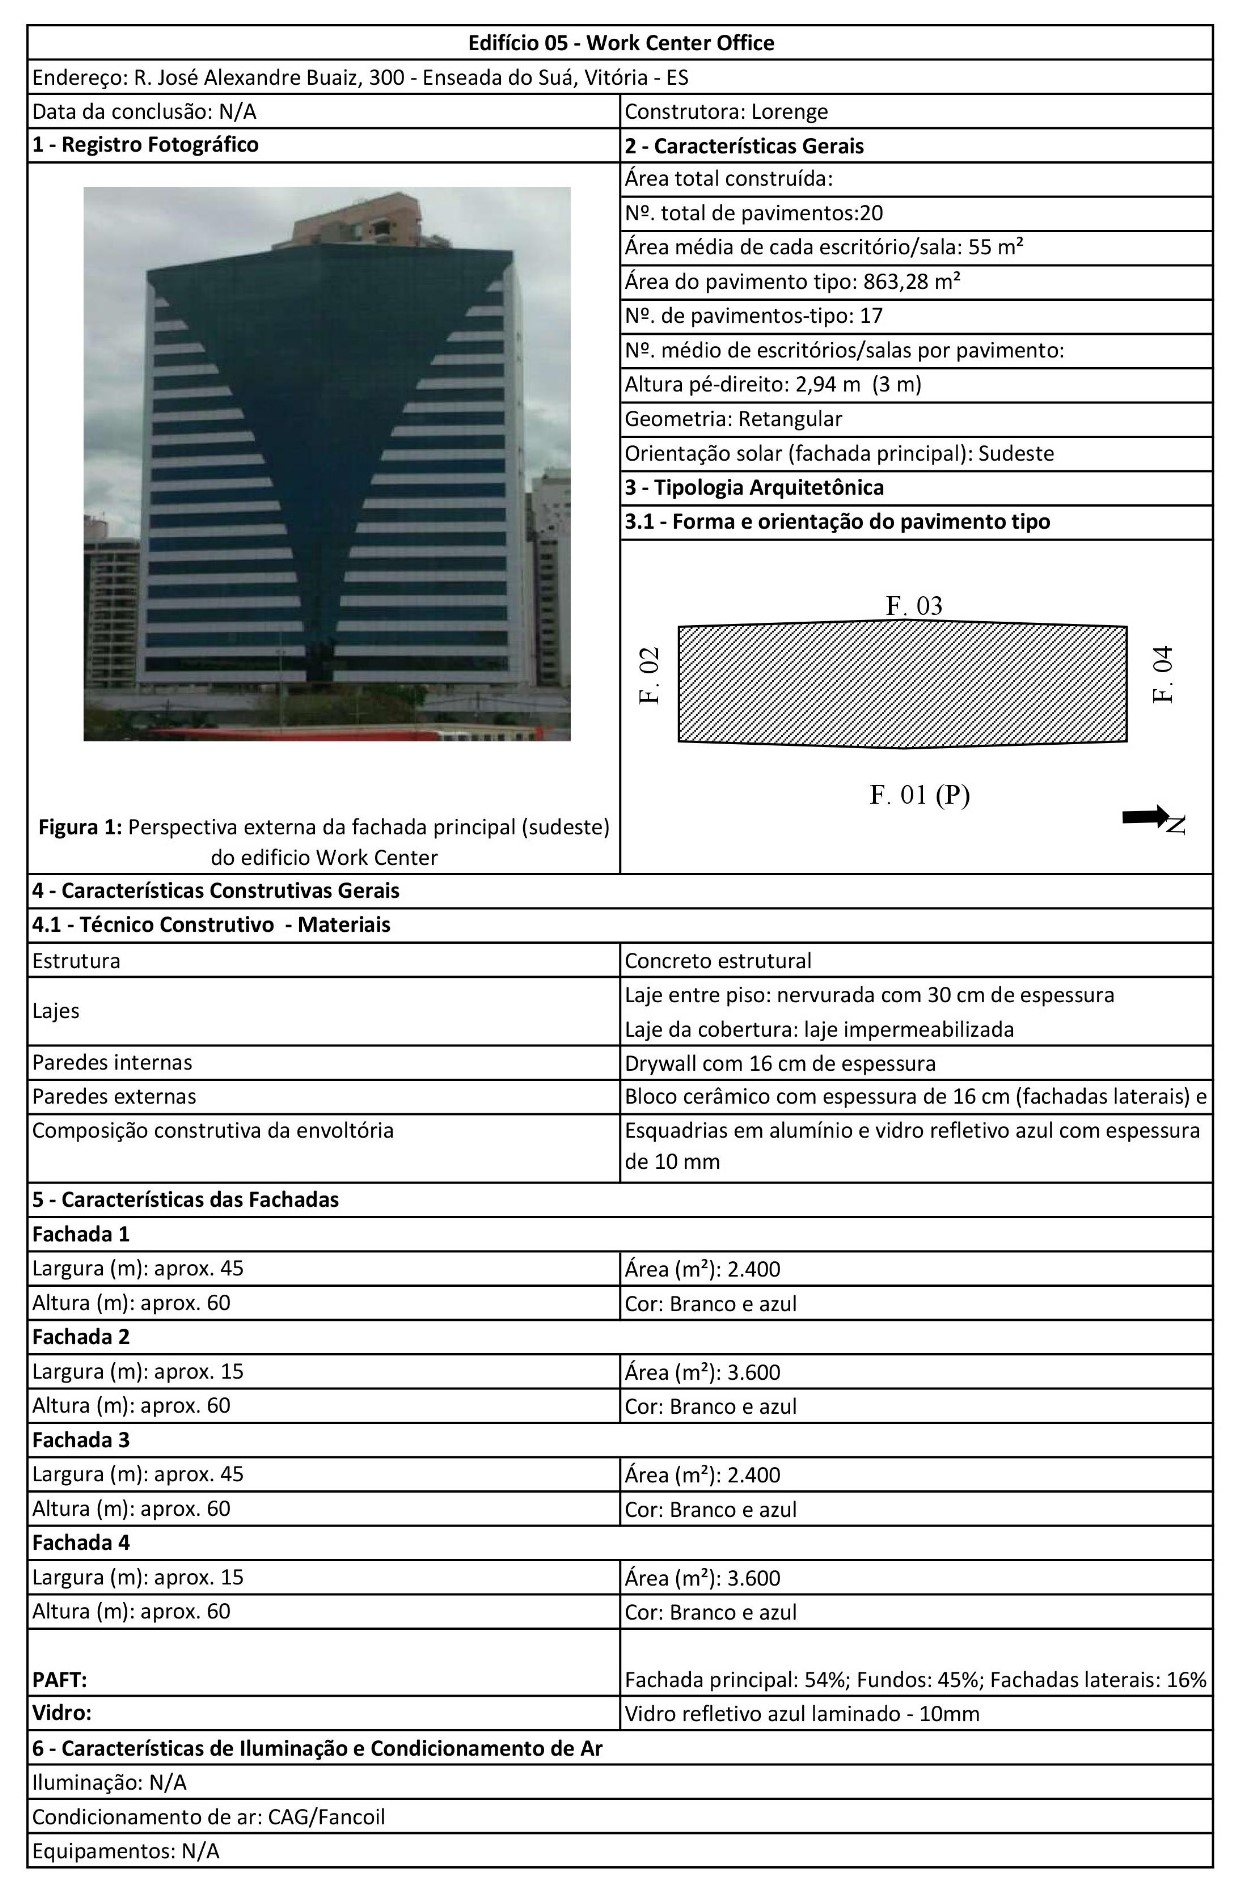
\includegraphics[width=\textwidth]{figures/appendices/edificio05.jpg}
    \end{tabular}
\end{table}
\pagebreak
\begin{table}[H]
    \centering
    \begin{tabular}{l}
        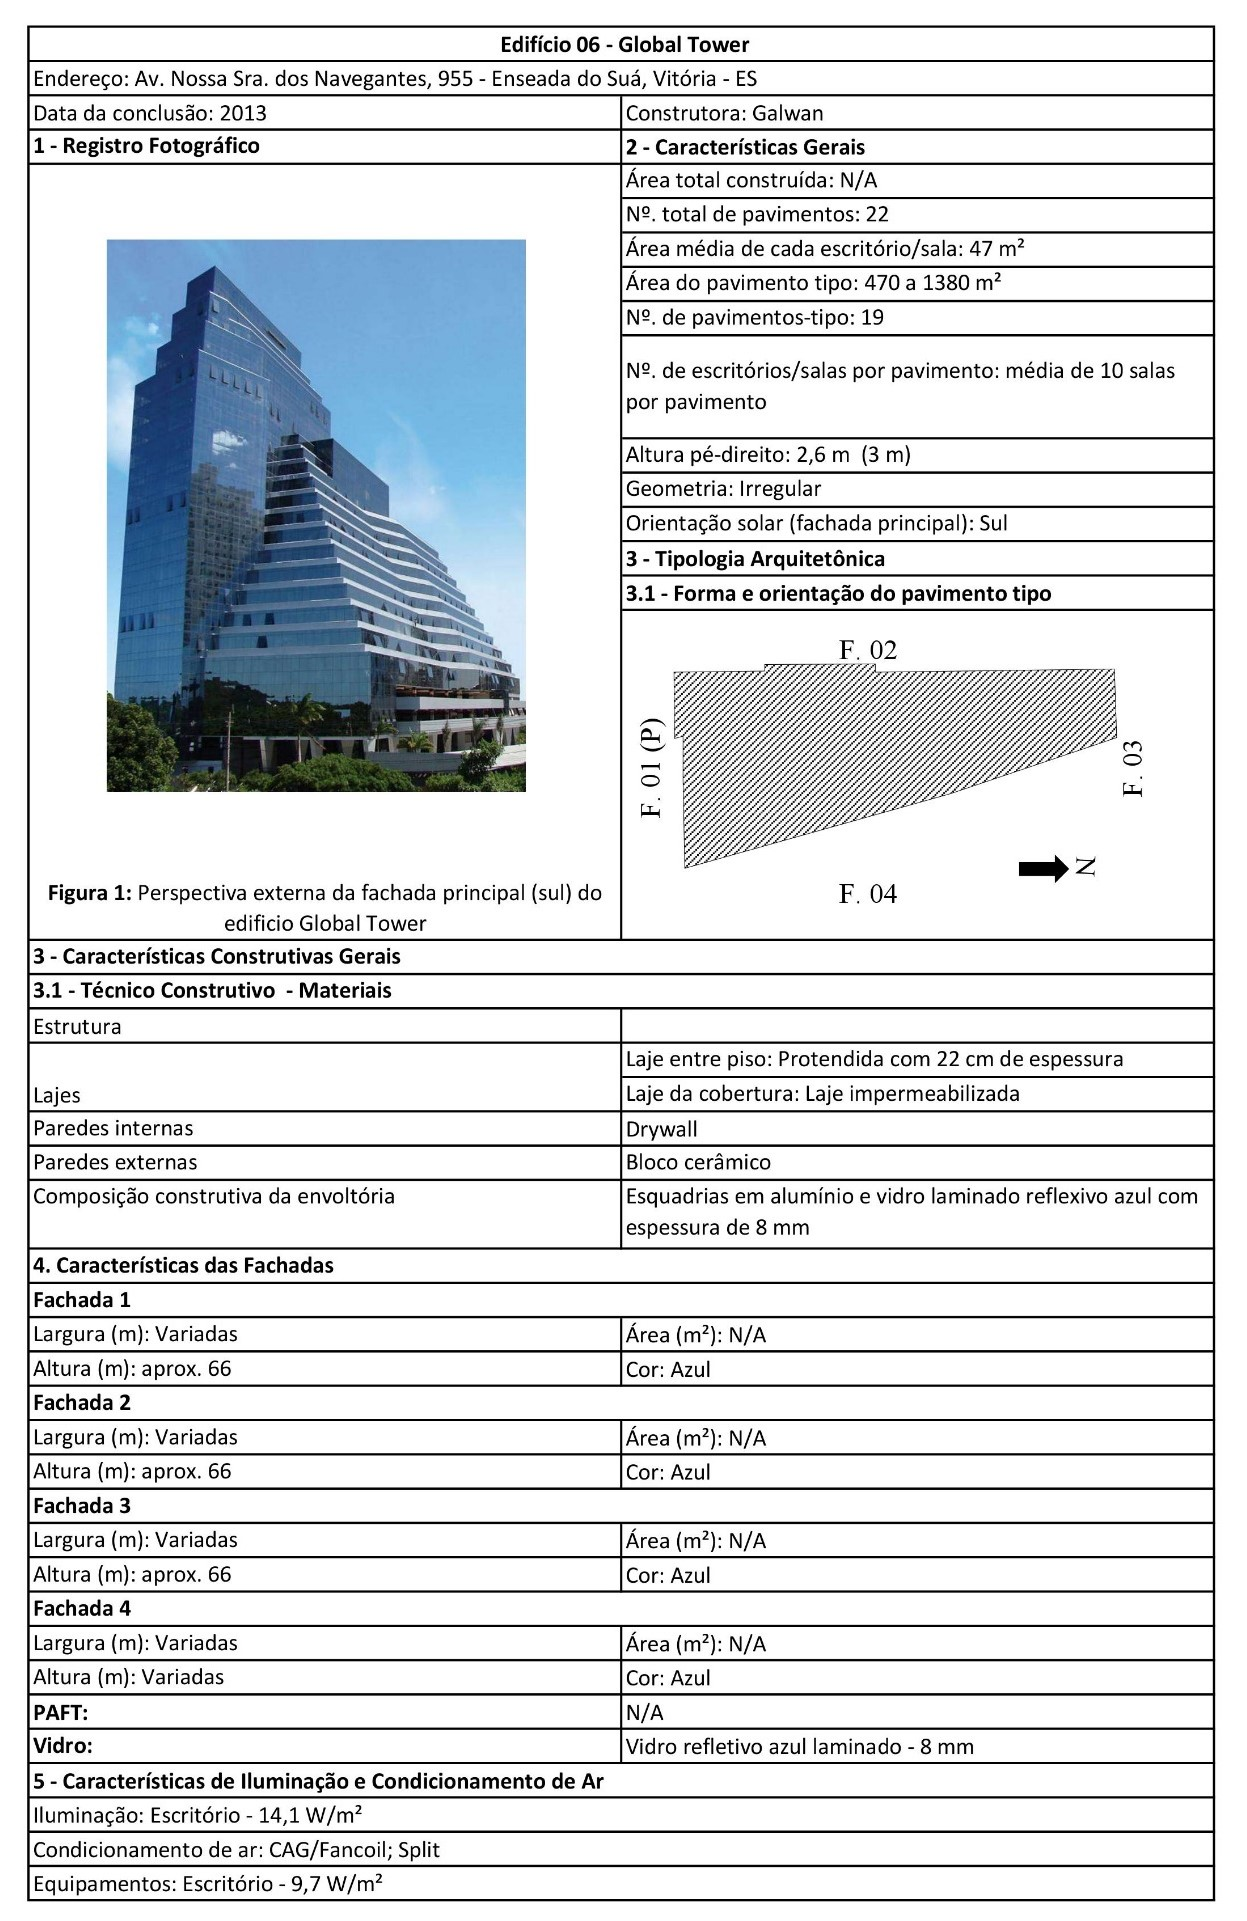
\includegraphics[width=\textwidth]{figures/appendices/edificio06.jpg}
    \end{tabular}
\end{table}
\pagebreak
\begin{table}[H]
    \centering
    \begin{tabular}{l}
        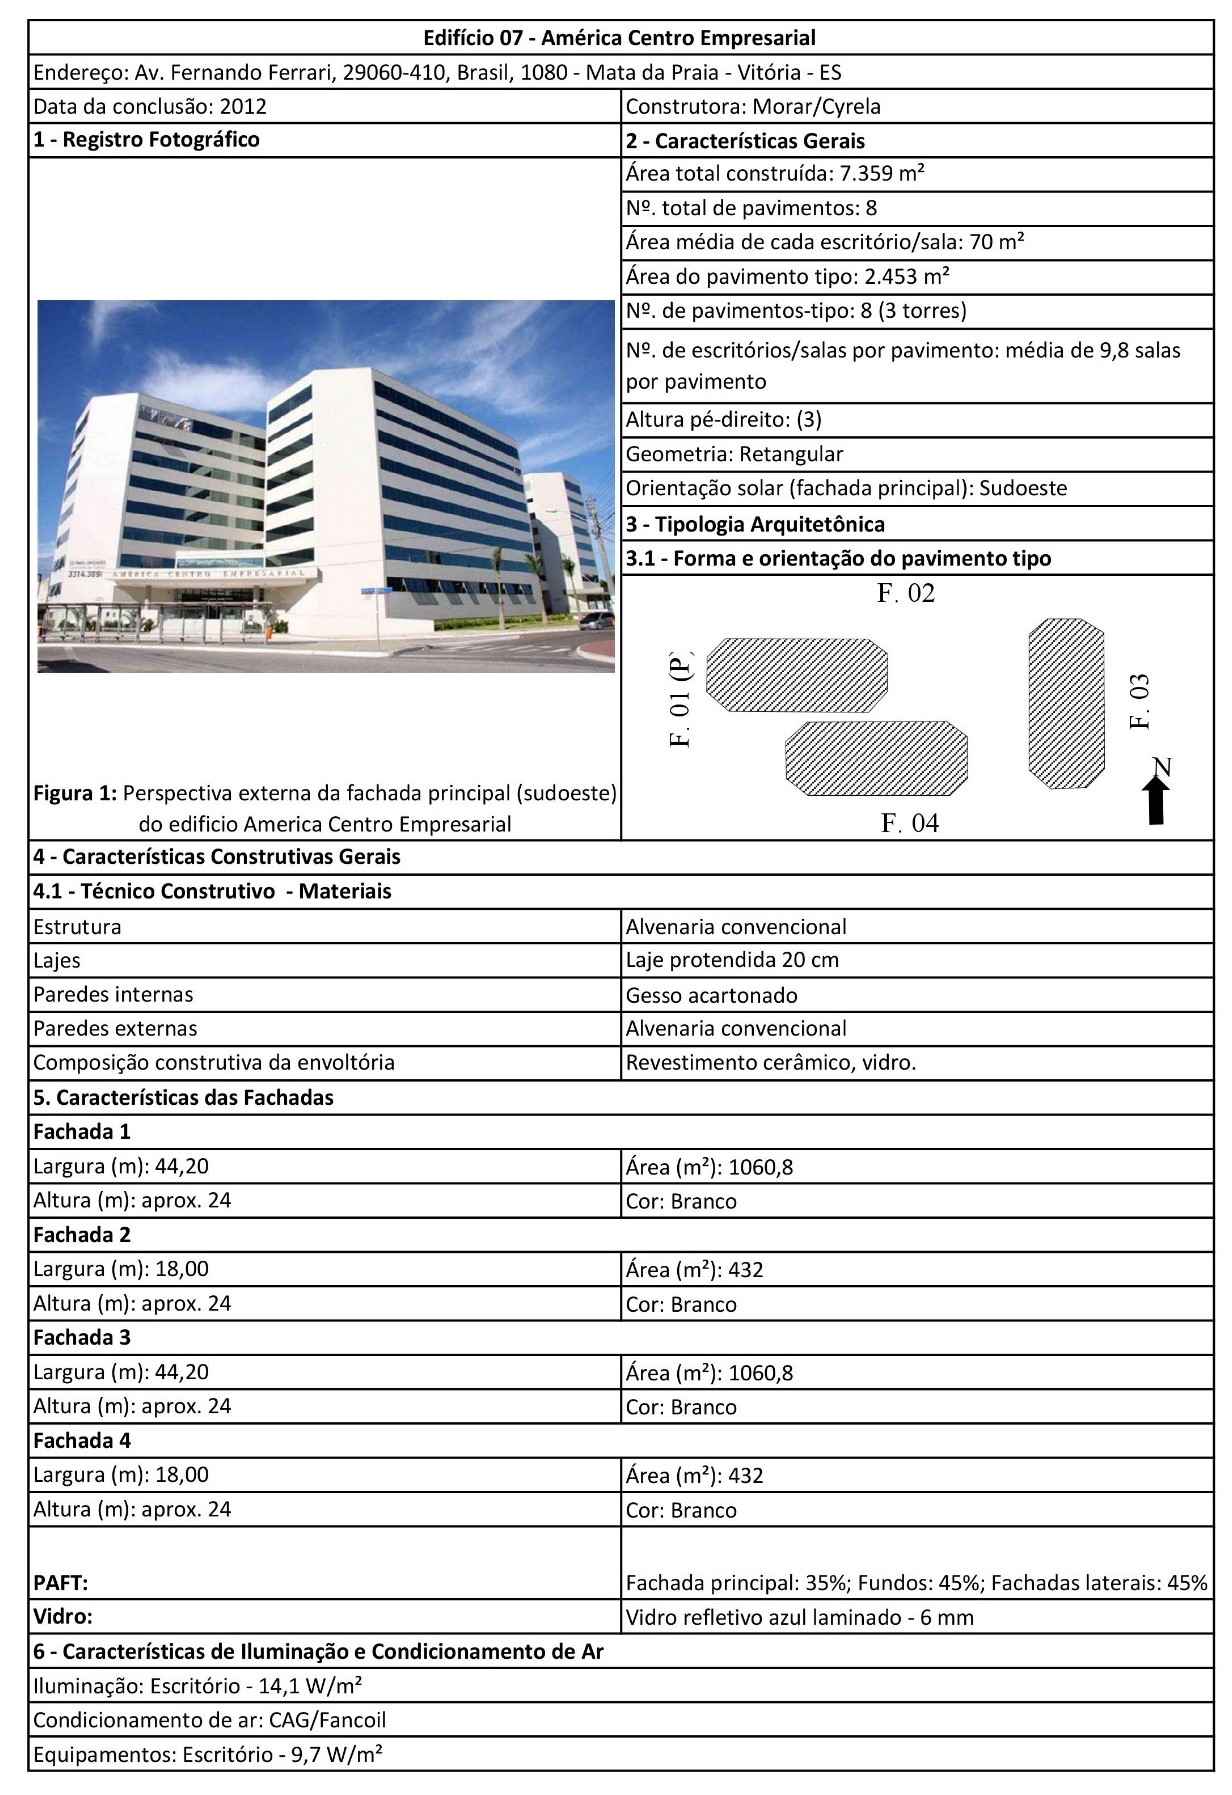
\includegraphics[width=\textwidth]{figures/appendices/edificio07.jpg}
    \end{tabular}
\end{table}
\pagebreak
\begin{table}[H]
    \centering
    \begin{tabular}{l}
        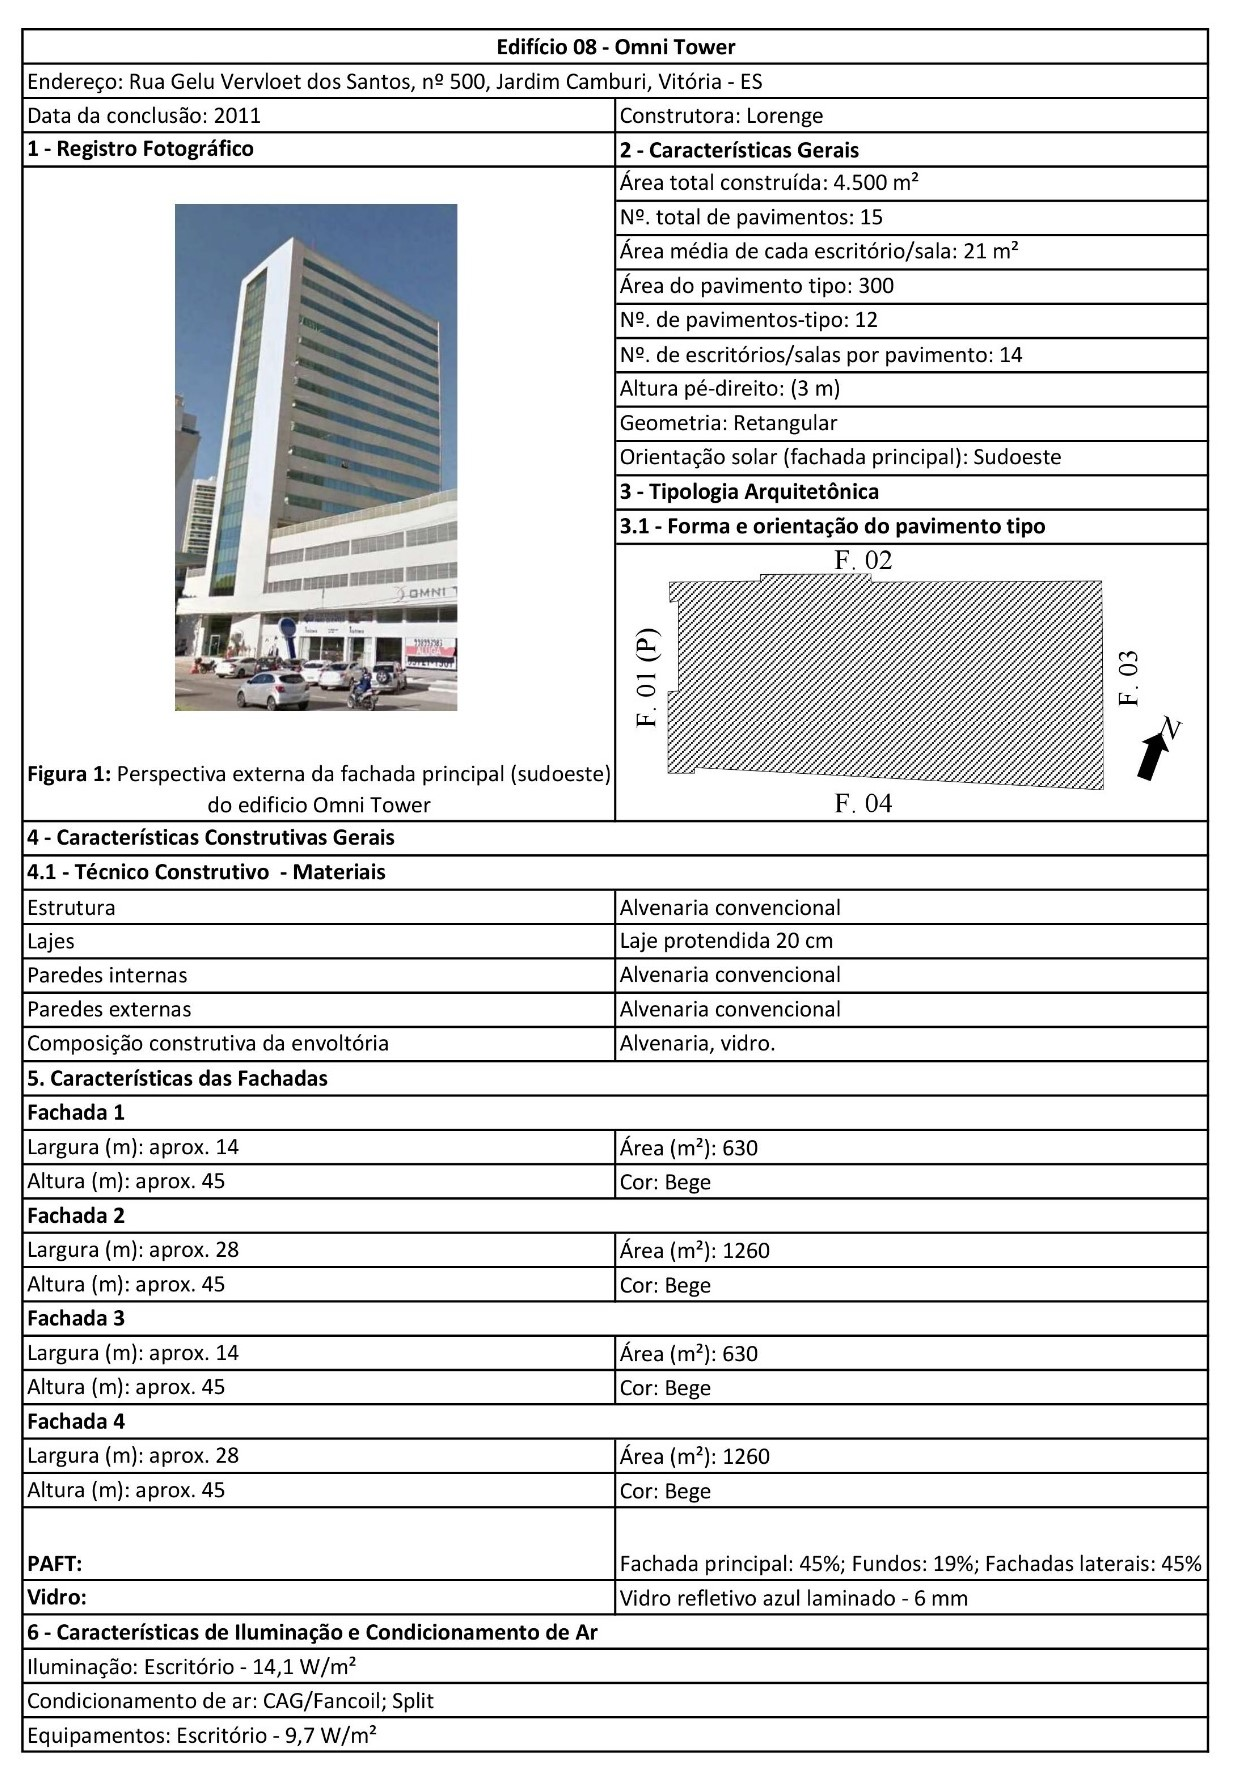
\includegraphics[width=\textwidth]{figures/appendices/edificio08.jpg}
    \end{tabular}
\end{table}
\pagebreak
\begin{table}[H]
    \centering
    \begin{tabular}{l}
        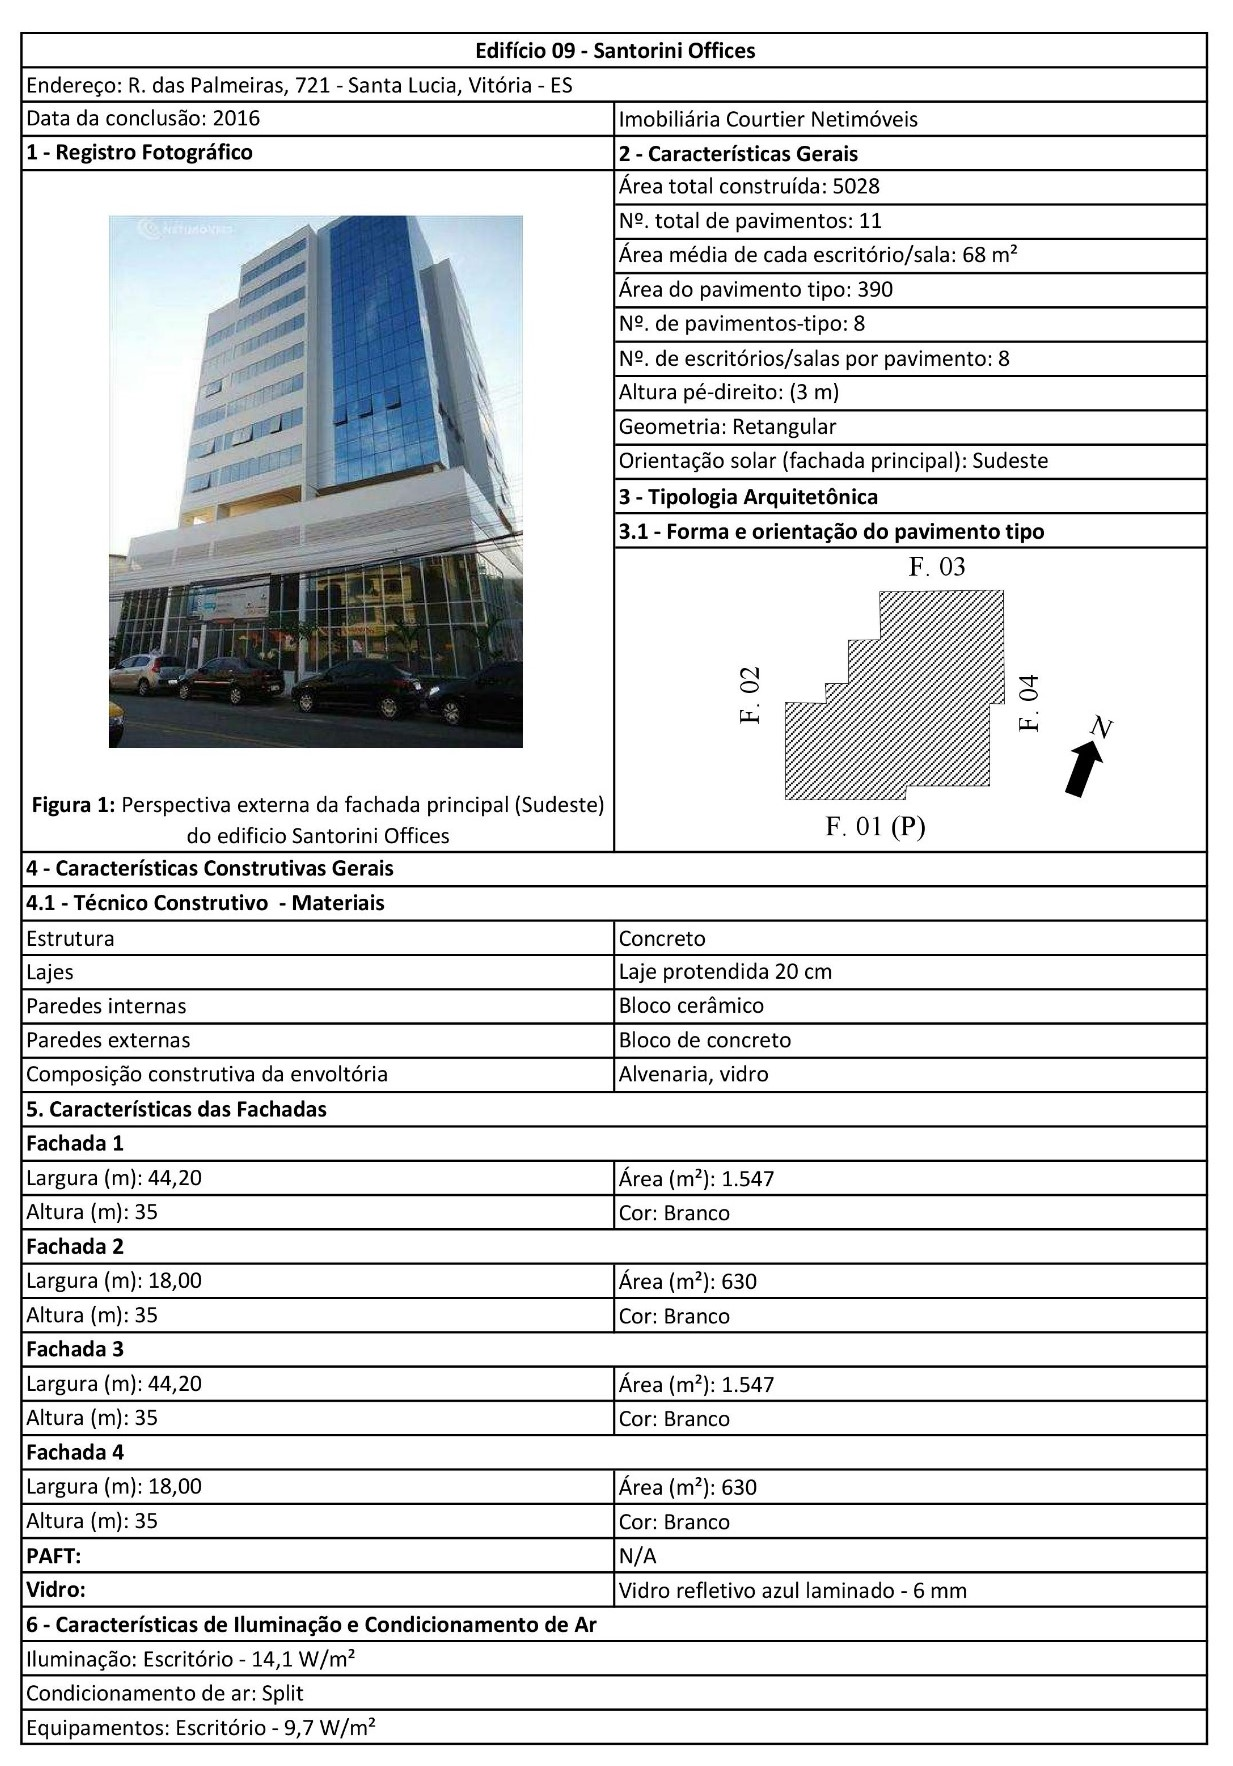
\includegraphics[width=\textwidth]{figures/appendices/edificio09.jpg}
    \end{tabular}
\end{table}
\pagebreak
\begin{table}[H]
    \centering
    \begin{tabular}{l}
        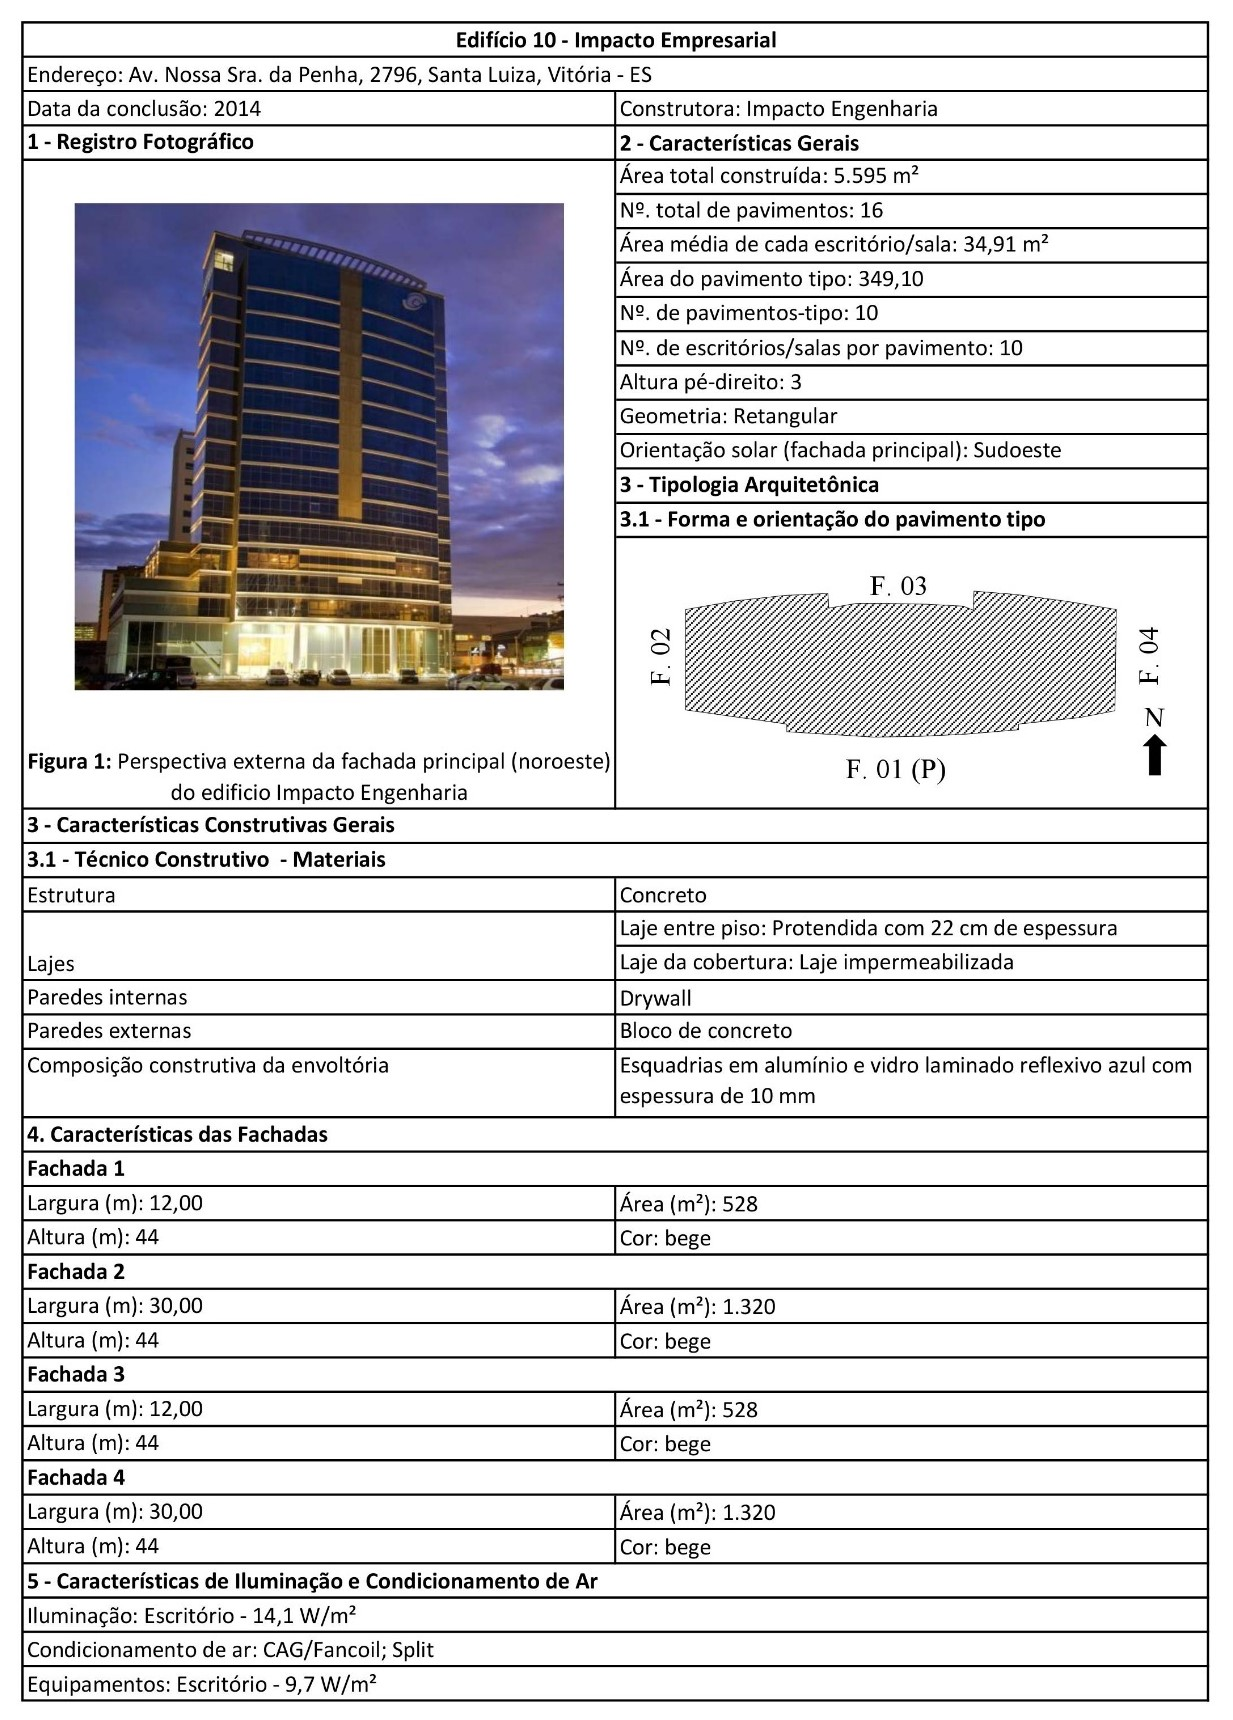
\includegraphics[width=\textwidth]{figures/appendices/edificio10.jpg}
    \end{tabular}
\end{table}
\vspace*{-0,5cm}
\subsection{Apêndice B}
\begin{table}[H]
    \centering
    \caption{Resultados de otimização para o modelo genérico de 8 pavimentos.}
    \begin{tabular}{l}
        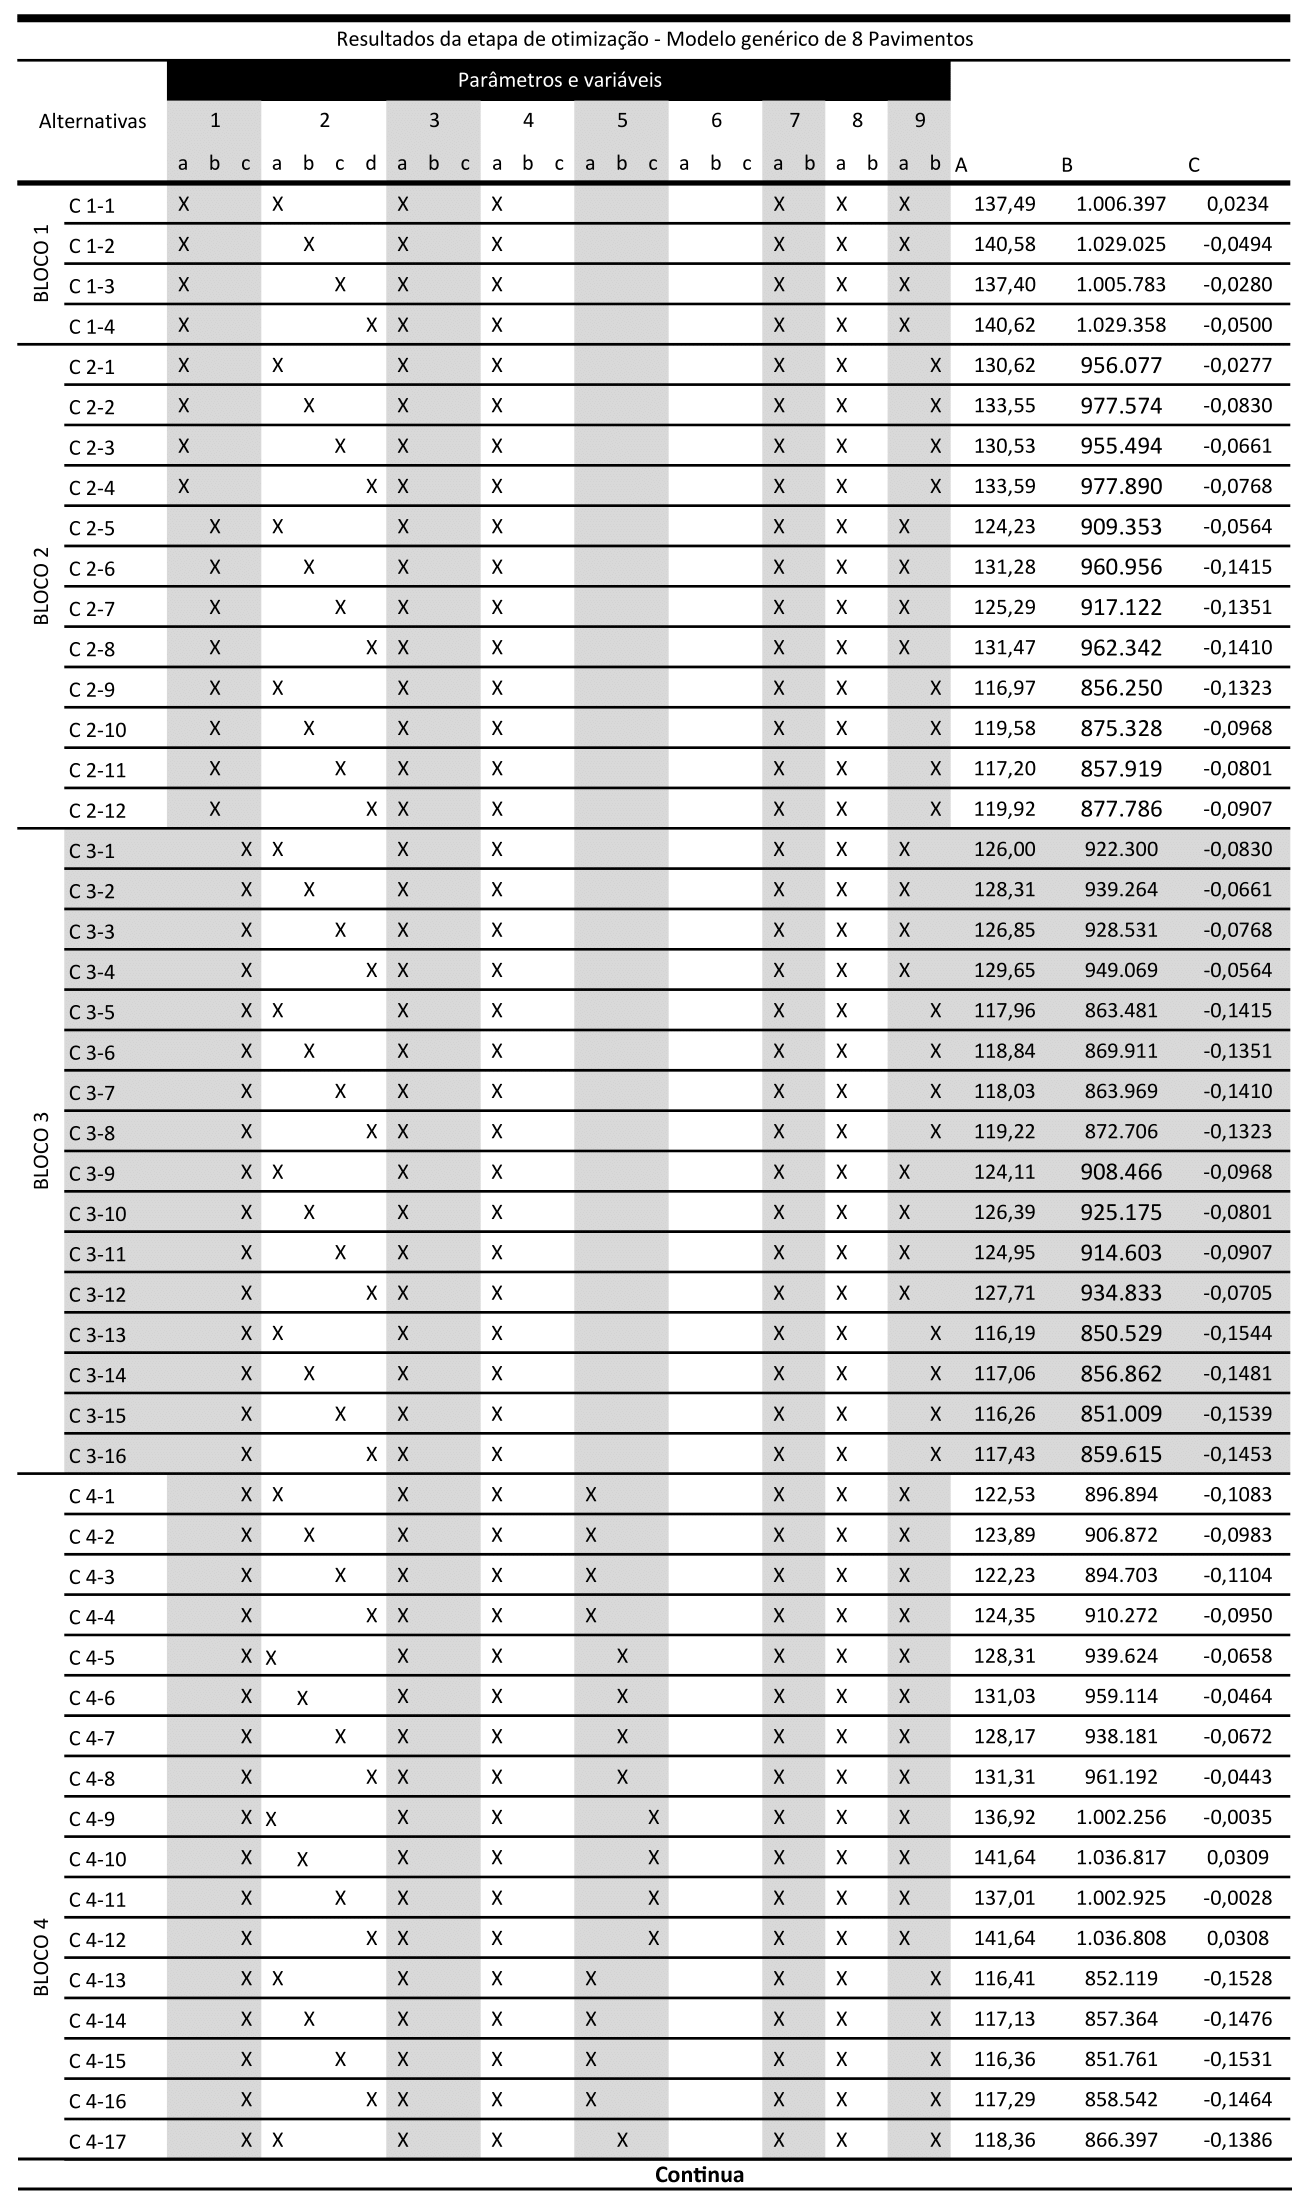
\includegraphics[width=0.85\textwidth]{figures/appendices/tabela01.png}
    \end{tabular}
    \label{tab:19}
\end{table}
\pagebreak
\begin{table}[H]
    \centering
    \begin{tabular}{l}
        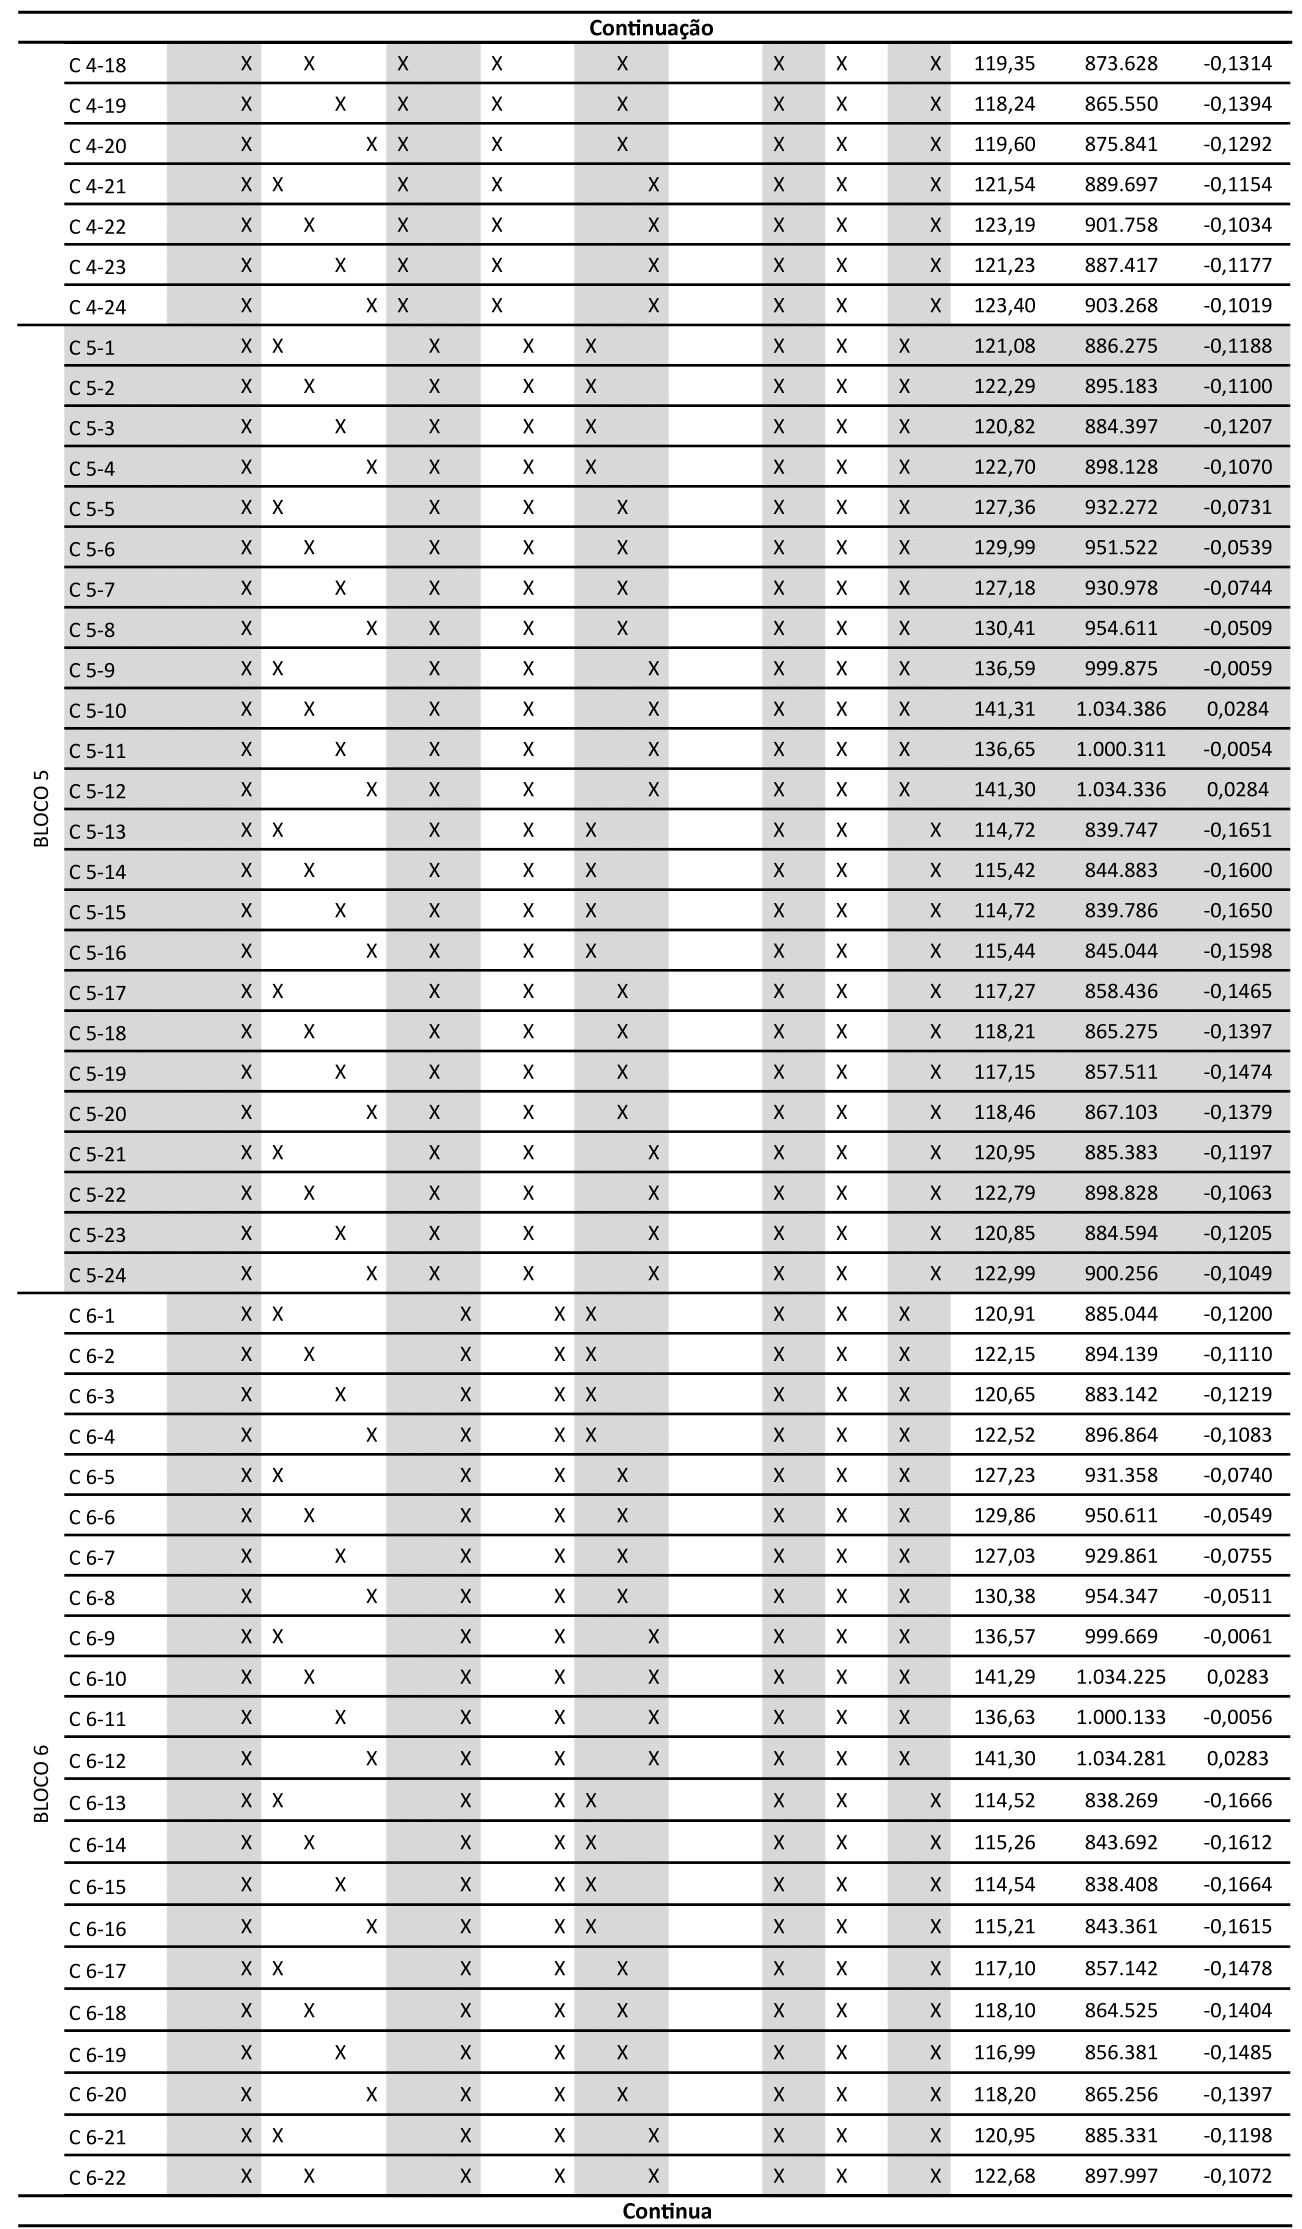
\includegraphics[width=0.9\textwidth]{figures/appendices/tabela02.png}
    \end{tabular}
\end{table}
\pagebreak
\begin{table}[H]
    \centering
    \begin{tabular}{l}
        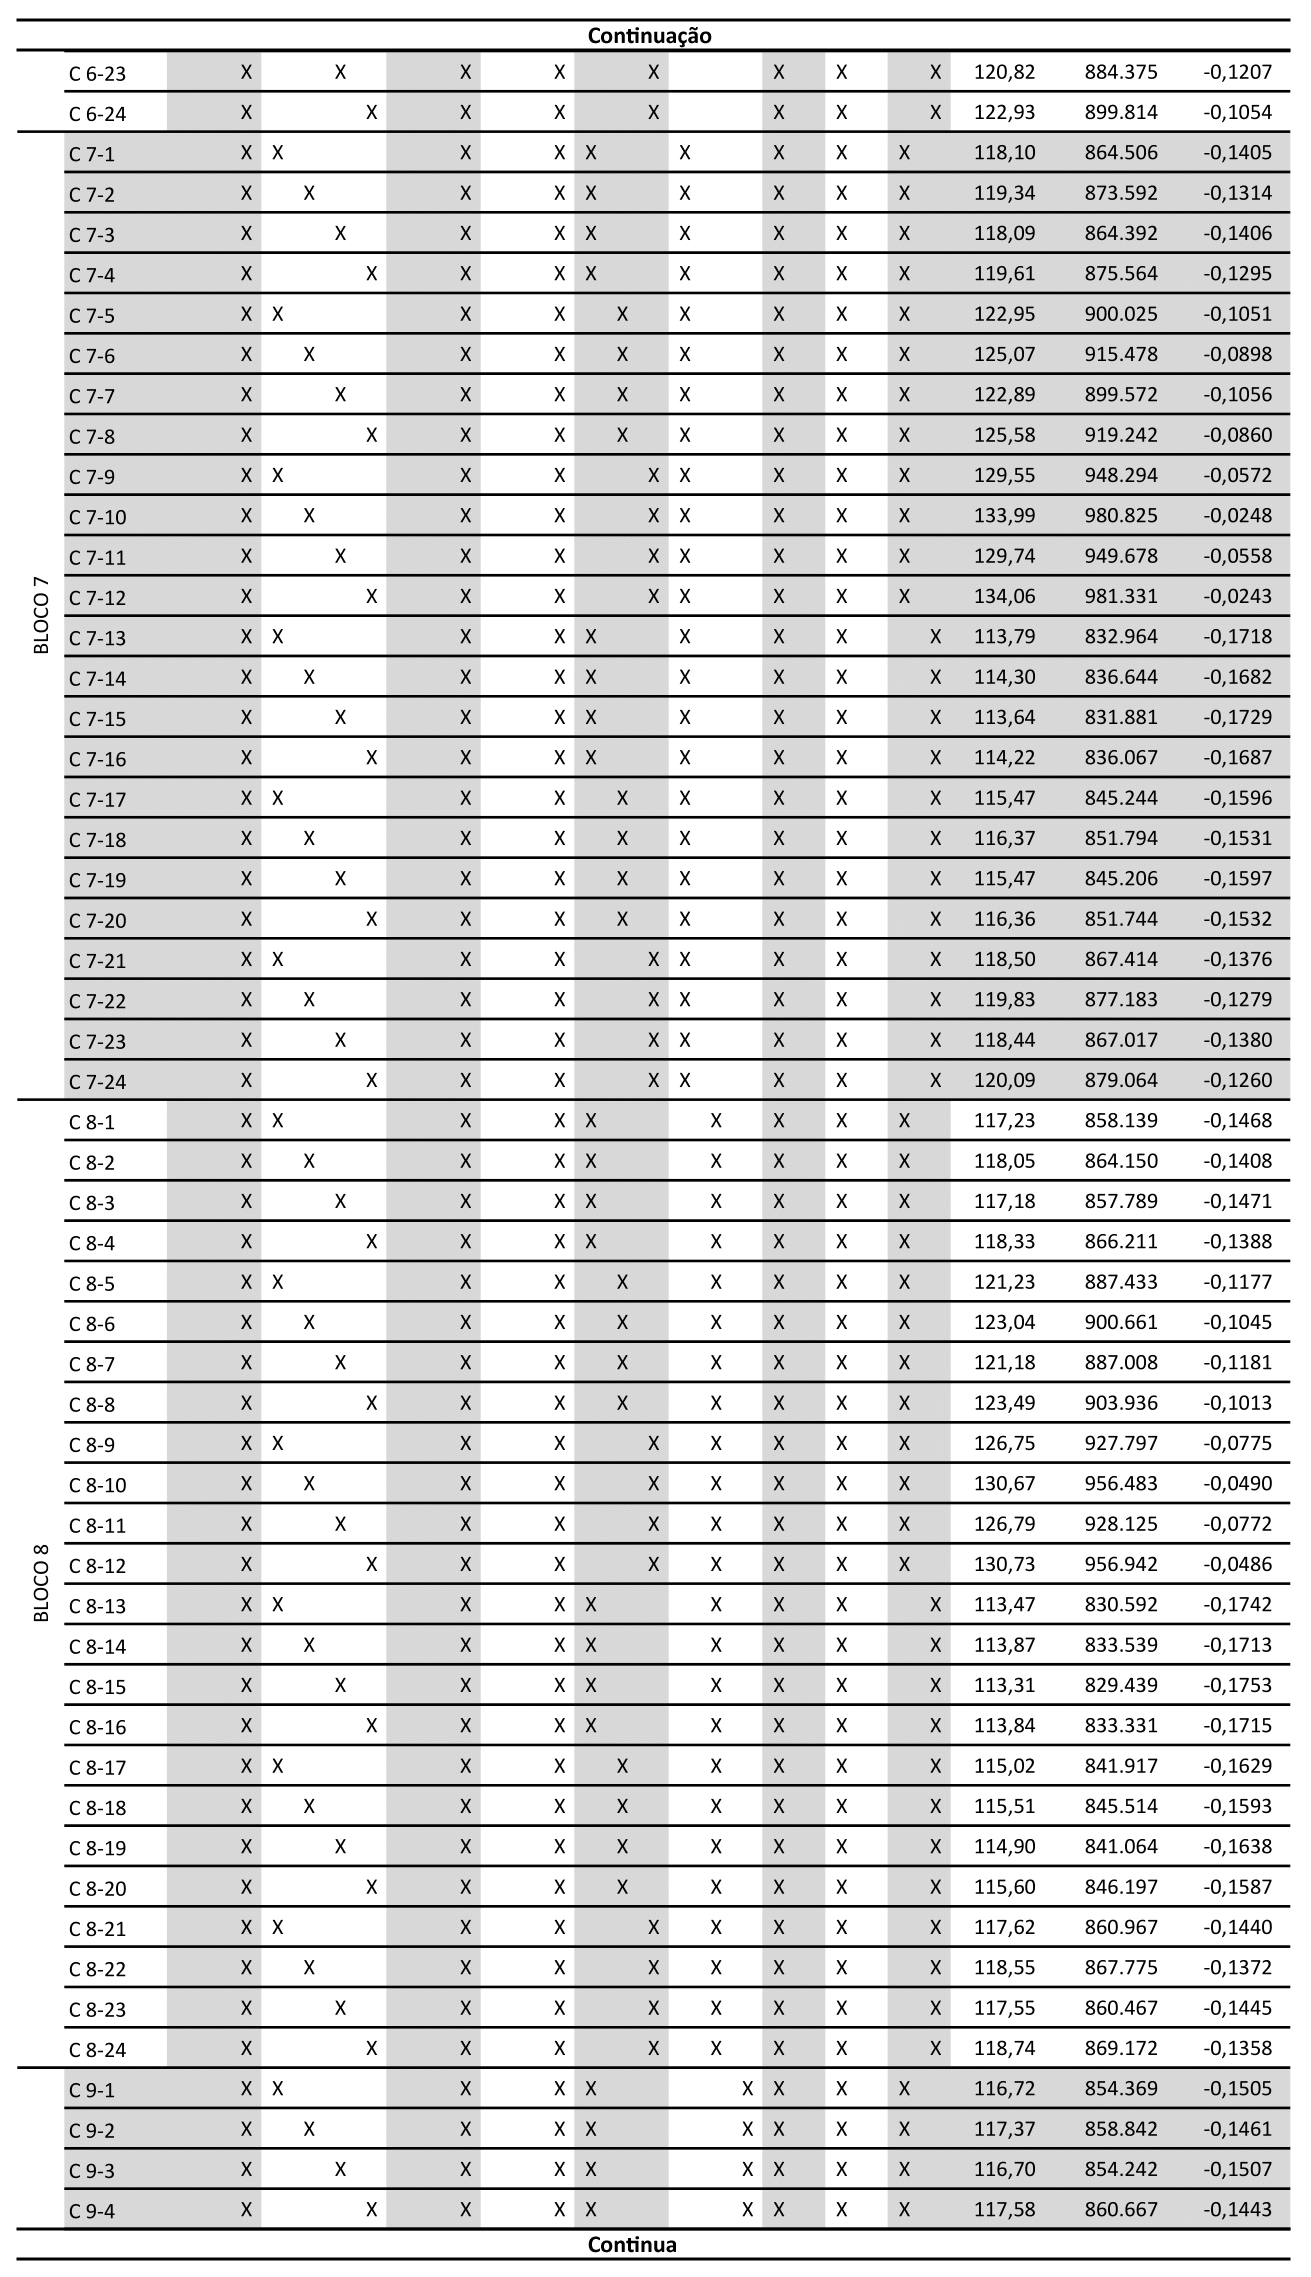
\includegraphics[width=0.9\textwidth]{figures/appendices/tabela03.png}
    \end{tabular}
\end{table}
\pagebreak
\begin{table}[H]
    \centering
    \begin{tabular}{l}
        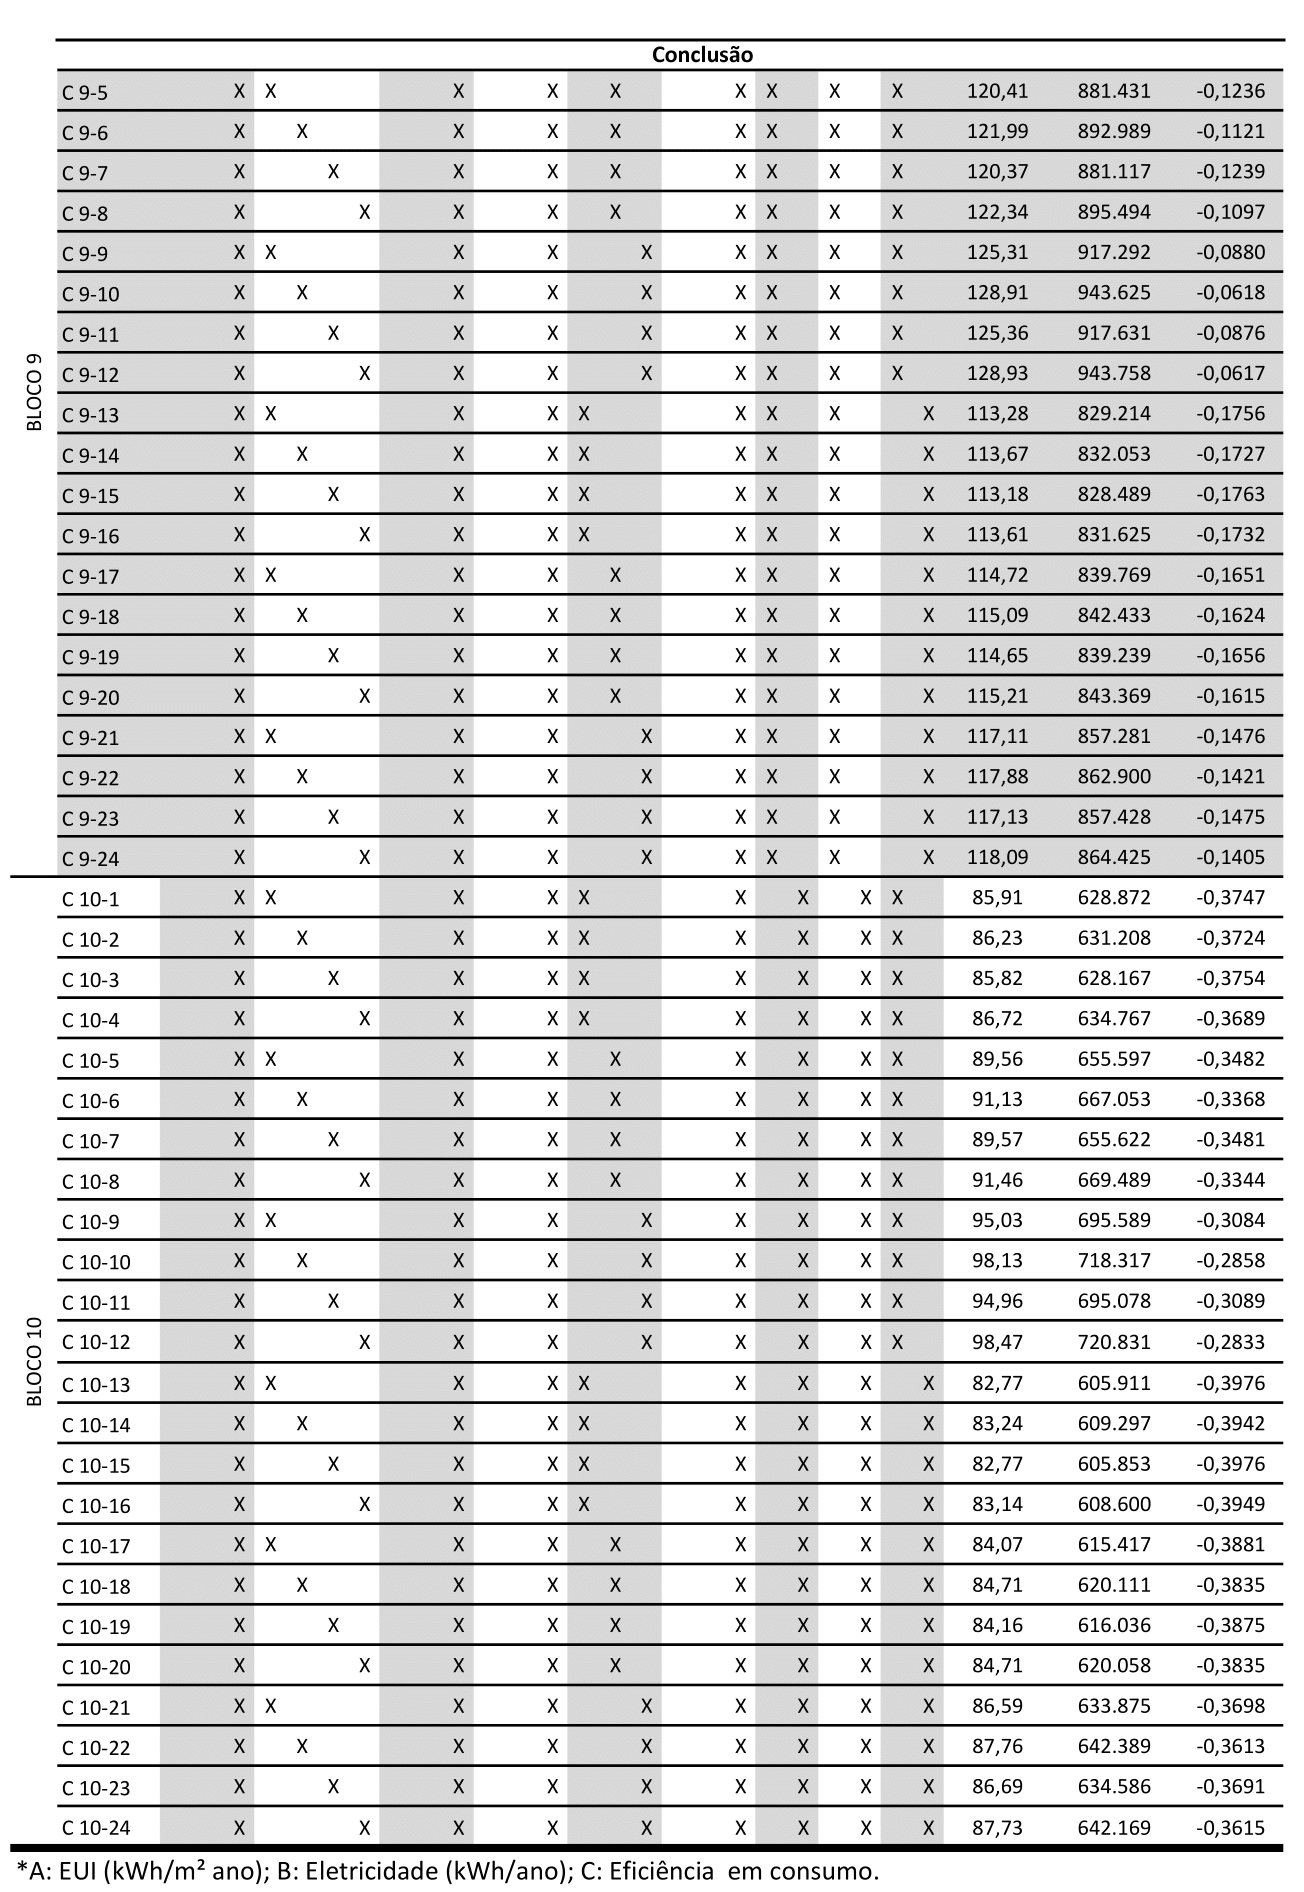
\includegraphics[width=\textwidth]{figures/appendices/tabela04.png}
    \end{tabular}
\end{table}
\subsection{Apêndice C}
\begin{table}[H]
    \centering
    \caption{Resultados de otimização para o modelo genérico de 19 pavimentos.}
    \begin{tabular}{l}
        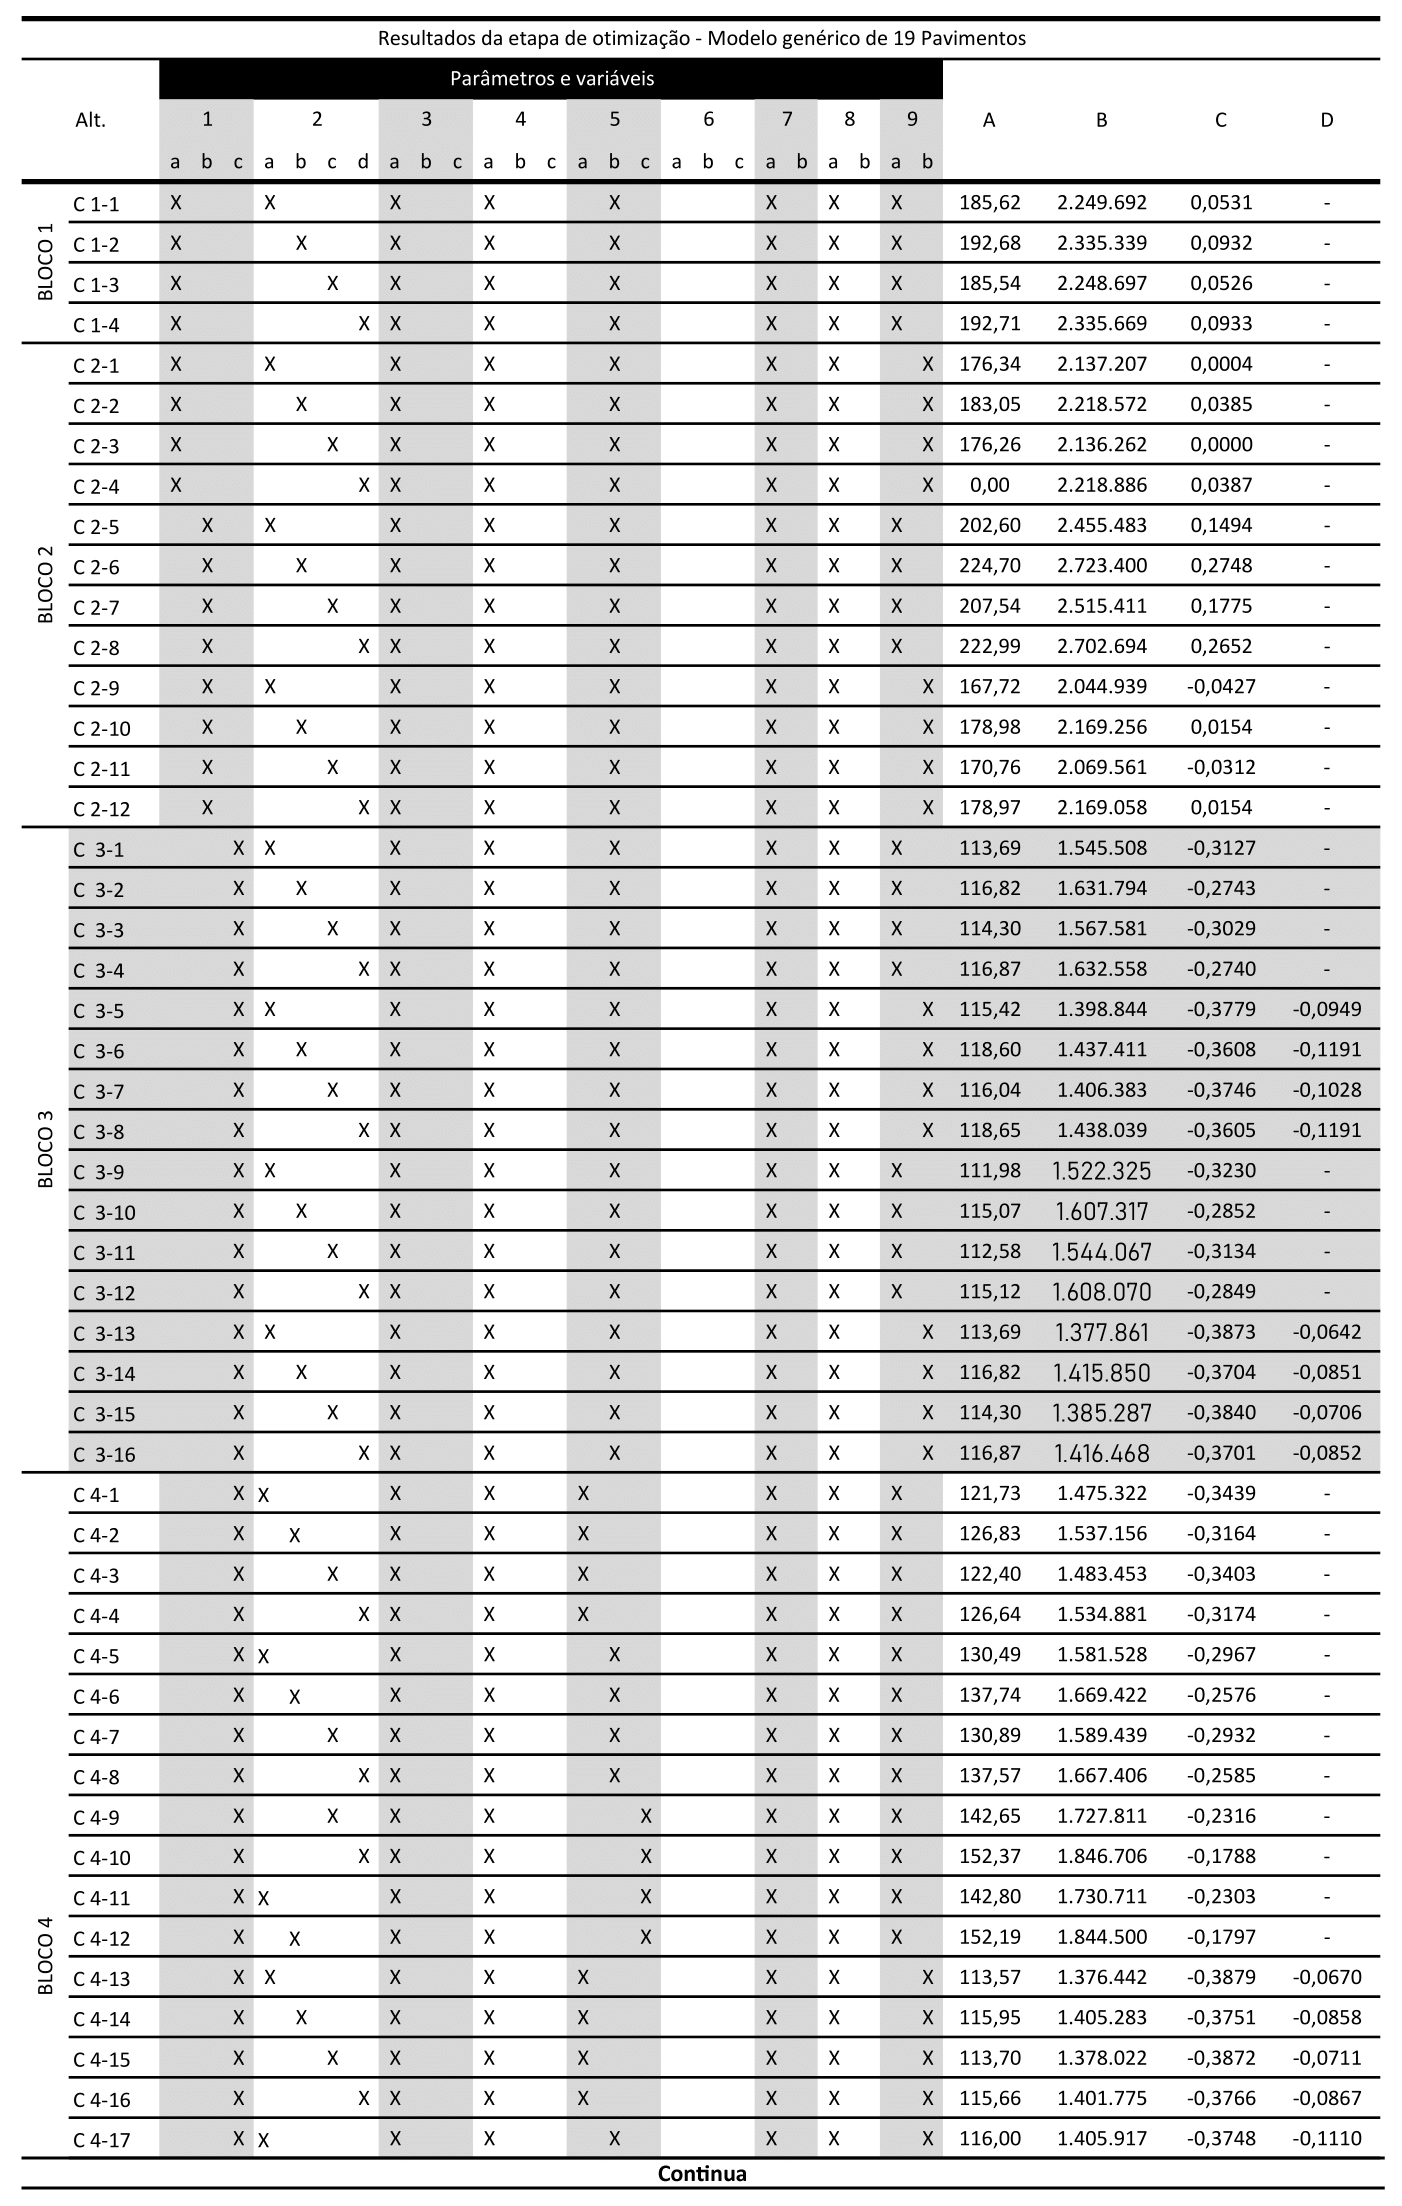
\includegraphics[width=0.9\textwidth]{figures/appendices/tabela05.png}
    \end{tabular}
    \label{tab:20}
\end{table}
\pagebreak
\begin{table}[H]
    \centering
    \begin{tabular}{l}
        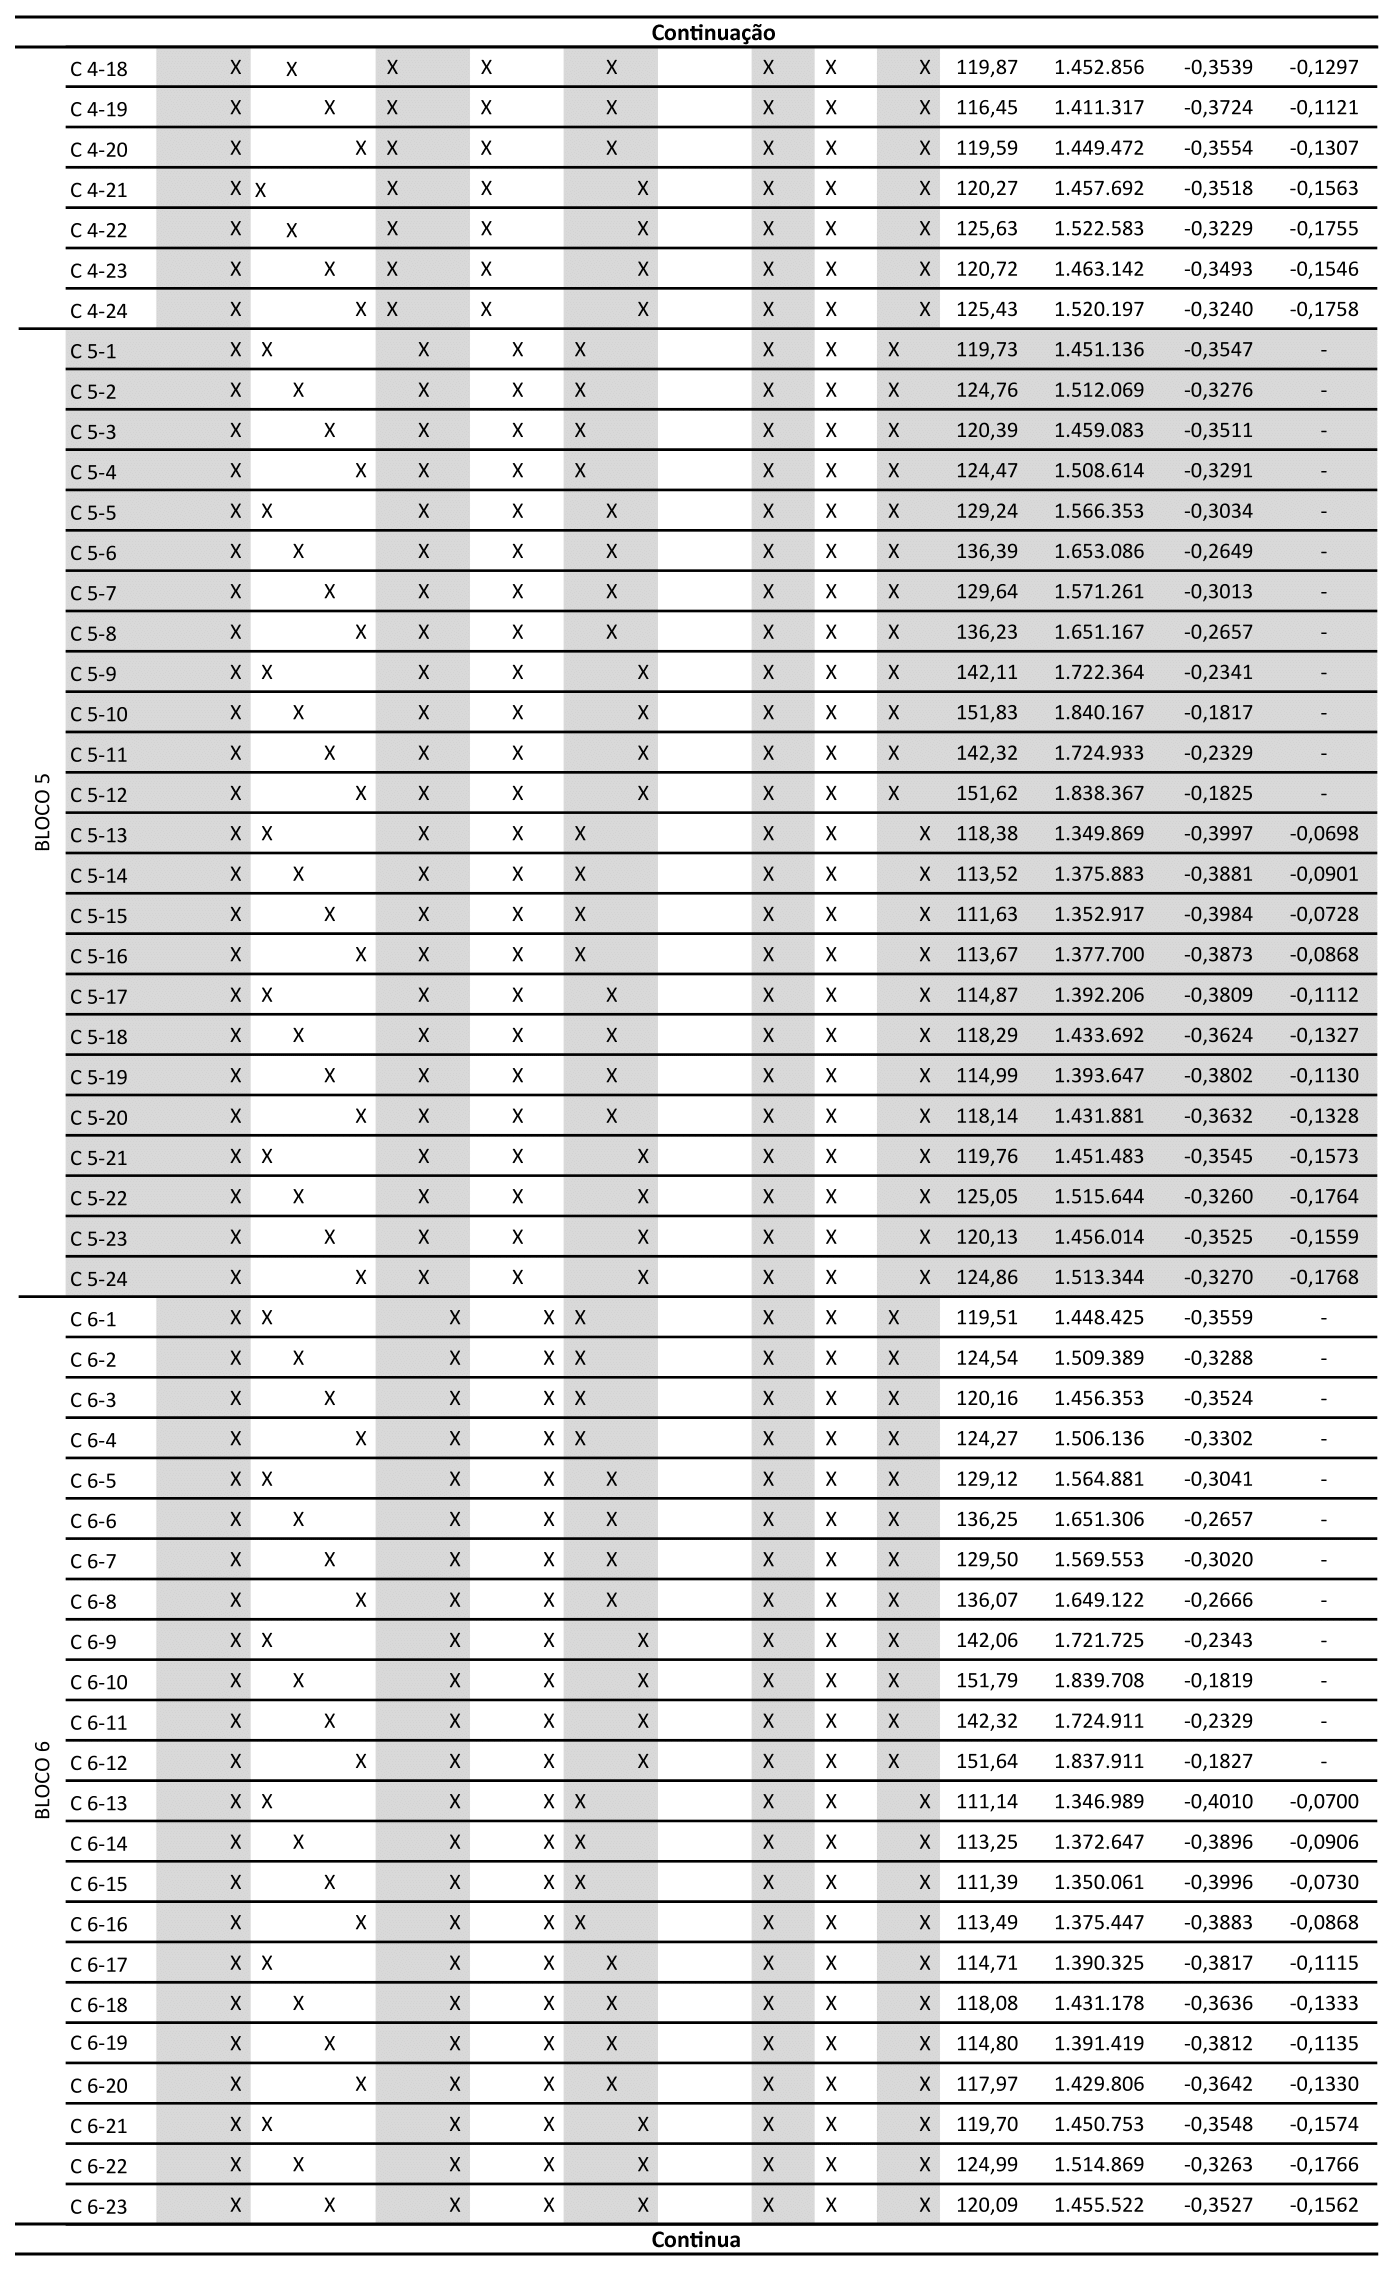
\includegraphics[width=0.9\textwidth]{figures/appendices/tabela06.png}
    \end{tabular}
\end{table}
\pagebreak
\begin{table}[H]
    \centering
    \begin{tabular}{l}
        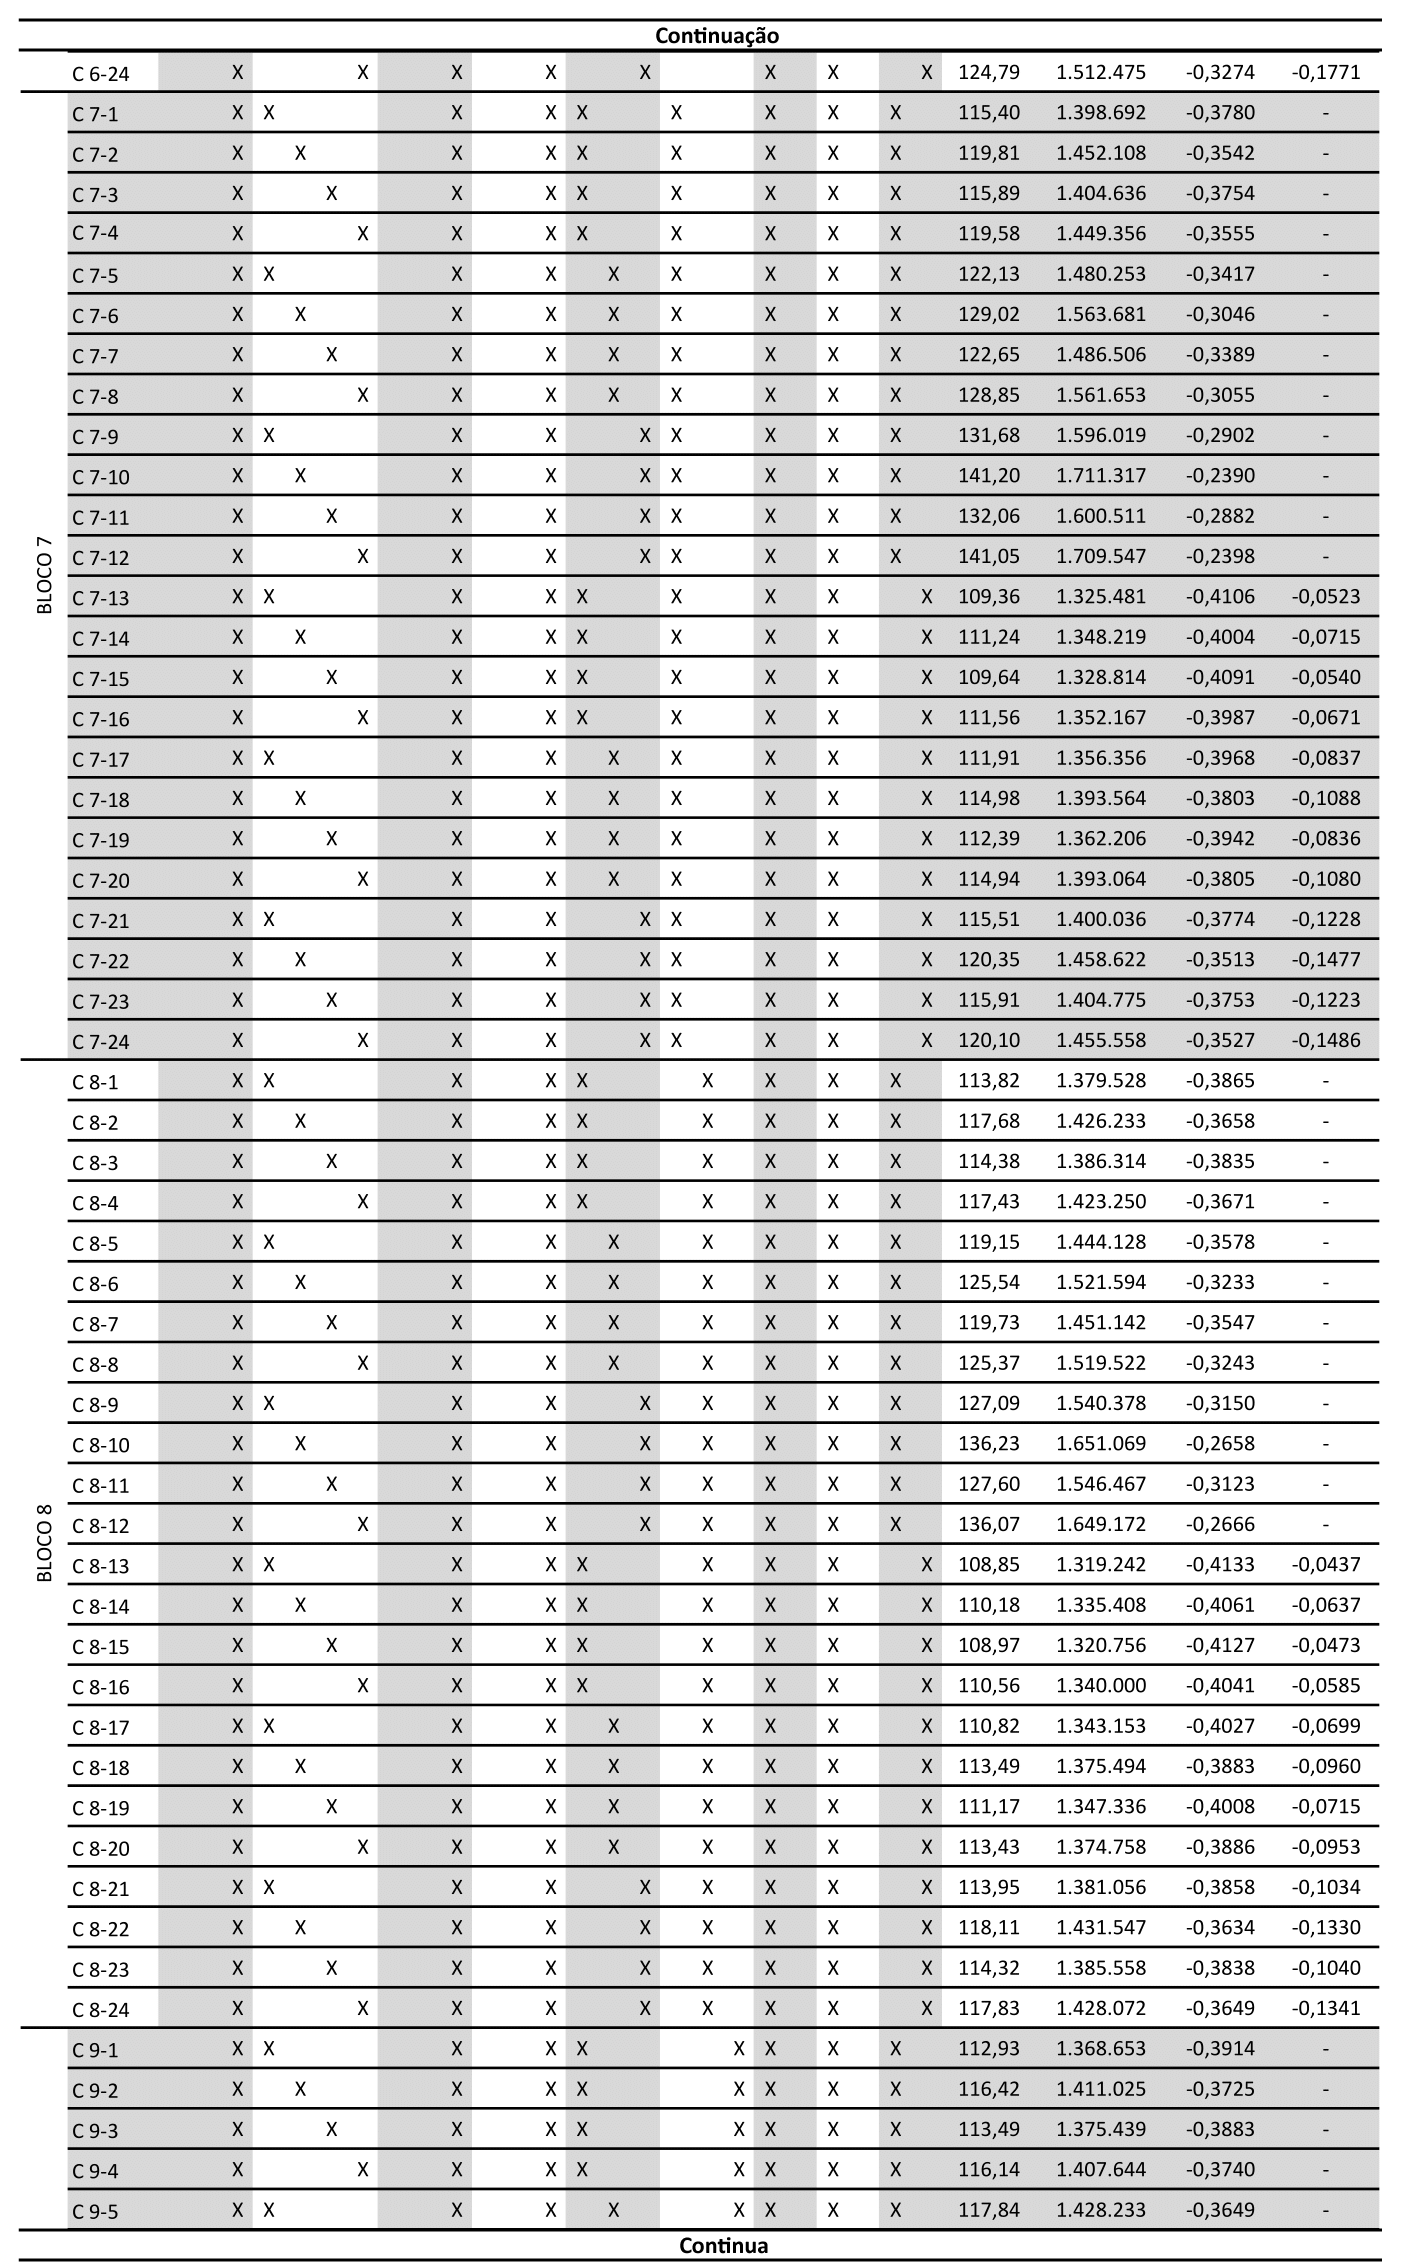
\includegraphics[width=0.9\textwidth]{figures/appendices/tabela07.png}
    \end{tabular}
\end{table}
\pagebreak
\begin{table}[H]
    \centering
    \begin{tabular}{l}
        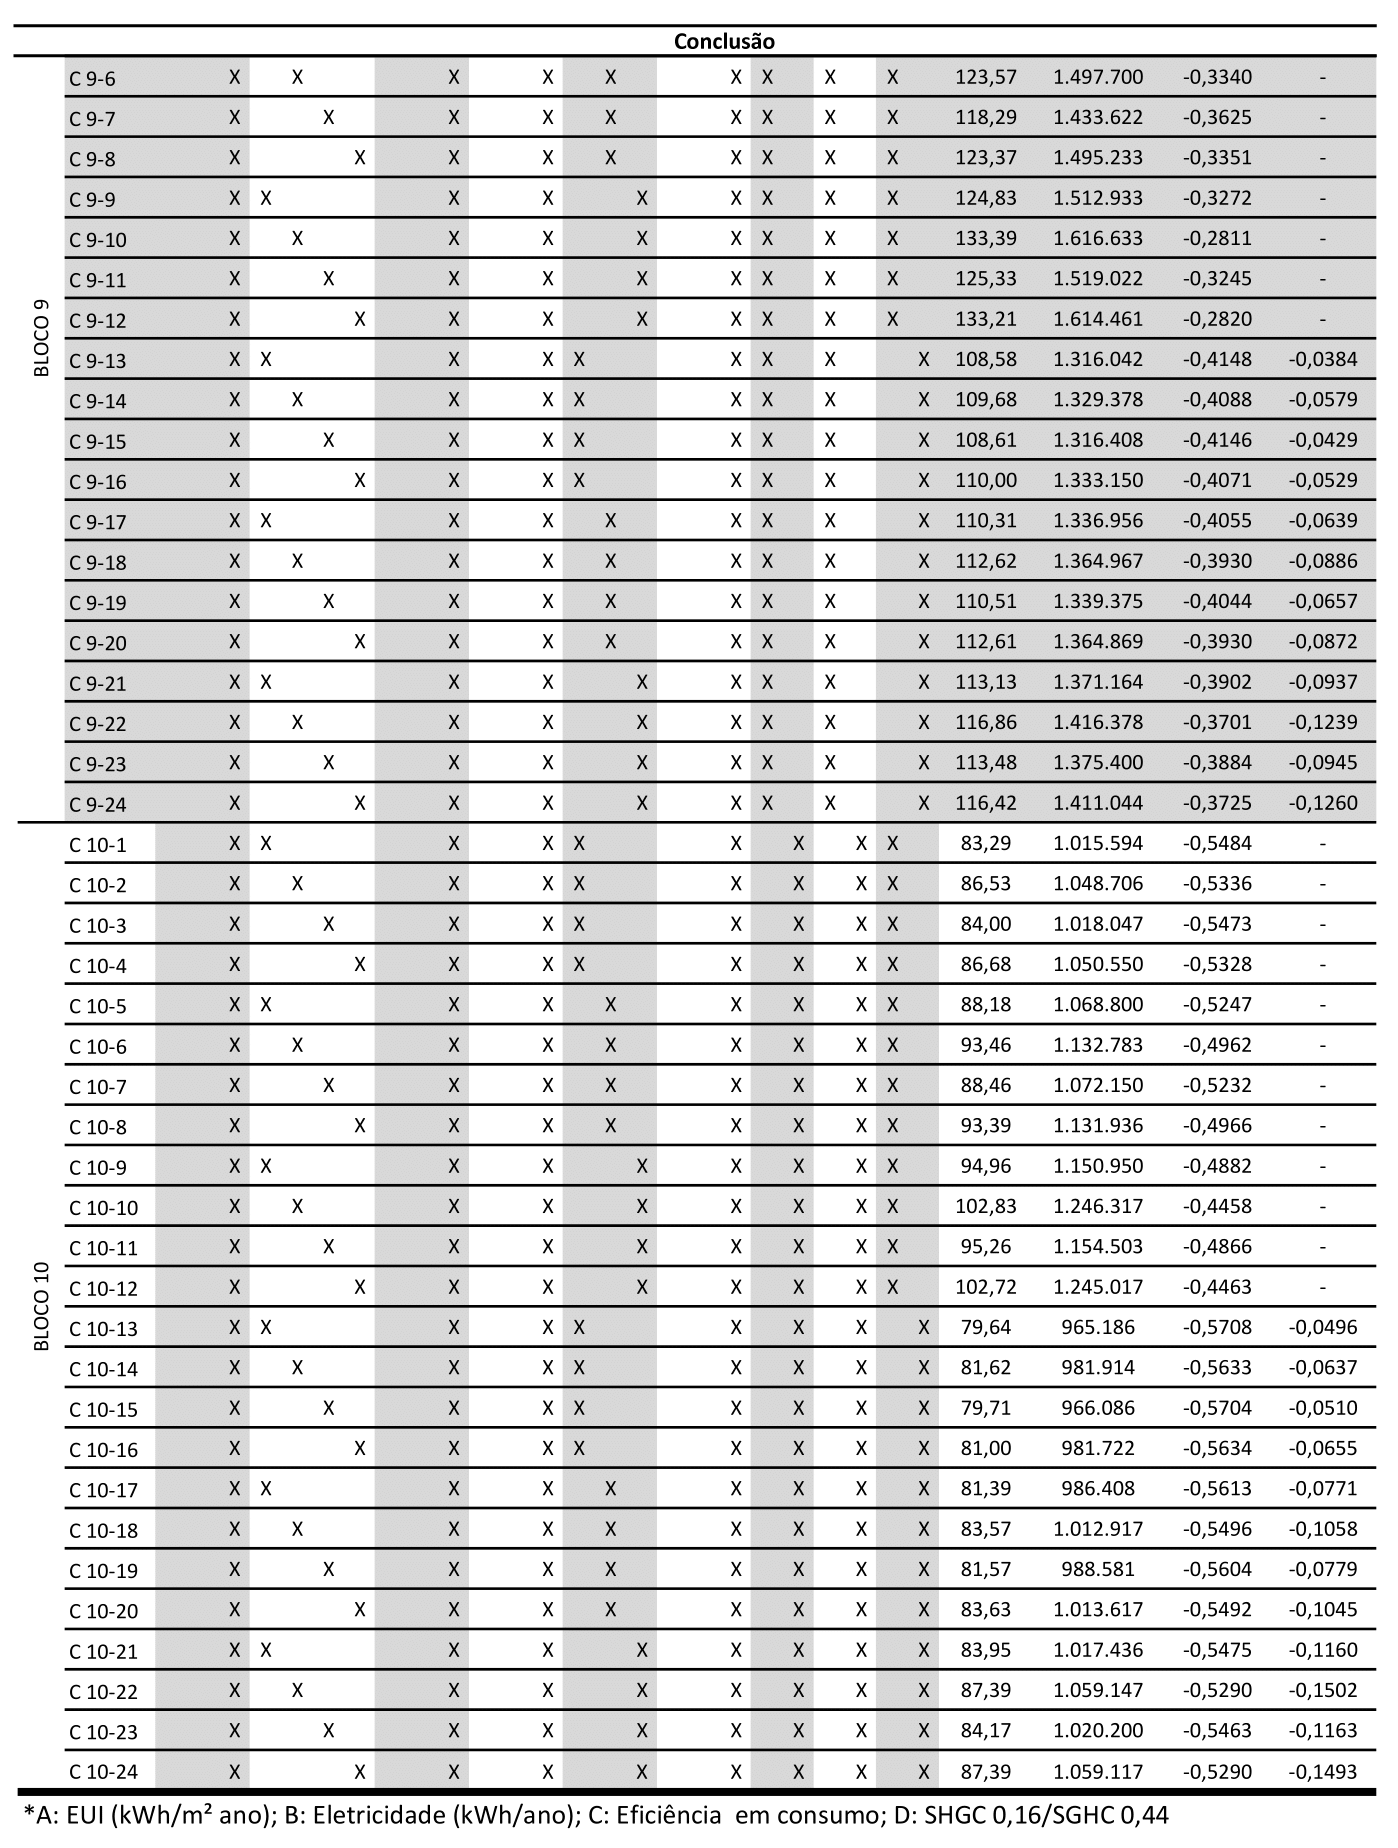
\includegraphics[width=0.9\textwidth]{figures/appendices/tabela08.png}
    \end{tabular}
\end{table}